\chapter{Pedagogy}\label{ch:pedagogy}
\noindent\emph{The following material is currently unpublished, but it is shared publicly in a dedicated repository\footnote{https://github.com/FoxFortino/SaturnineQuail-pedagogy}. Our team (myself, Dr. Federica Bianco, and Dr. Farid Qamar, who co-taught the course in 2024) is in discussion with publishers (\ie{} Princeton Press) to gauge their interest in turning these teaching materials into an undergraduate level textbook.}
\section{Introduction}\label{ch:pedagogy:intro}

\subsection{Motivation}
The previous chapters of this dissertation have focused on the development and application of machine learning methods for supernova classification. This chapter departs from direct astrophysical research to address a complementary endeavor: teaching data science.

Data science has become an essential skill across all scientific disciplines \cite{hey_fourth_2009,porcu_data_2026,vinuesa_decoding_2026,antonucci_data_2023,fu_ai_2026,hersh_beyond_2023,longo_data_2014,kang_cultivating_2026,bednarowska-michaiel_bringing_2026,zarefard_essential_2024,dong_are_2026,gunklach_beyond_2025}. The ability to analyze data, build models, and interpret results is no longer the exclusive purview of statisticians and computer scientists. These skills are increasingly expected of researchers and students in physics and astronomy, and any discipline that deals with data. Students arrive in the classroom with diverse academic backgrounds \cite{bednarowska-michaiel_bringing_2026,inproceedings}, widely varying levels of mathematical preparation and often only a modicum of programming experience or less; thus, the question asks itself: ``How do you teach data science?''

\subsection{Context}
The course ``Foundations of Data Science for Everyone'' (hereafter FDSE) was developed under National Science Foundation (NSF) award 2123264 ``Collaborative Research: HDR DSC: Delaware and Mid-Atlantic Data Science Corps'' (P.I. Bianco) to expand data science education at Lincoln University of Pennsylvania and Delaware State University. The materials presented in this chapter represent the culmination of several years of development. I first encountered this course as a teaching assistant, supporting Dr. Federica Bianco on this course for two semesters. I also served as her teaching assistant for a more advanced course covering similar material, ``Data Science for Physical Scientists.'' These courses gave me considerable experience on the `other side' of the classroom, which has let me develop my own professional opinions about teaching. The opportunity arose for me to be the primary instructor for this course in the Fall of 2025. During my time as professor, I refined and personalized the materials based on my cumulative experience as a student, emphasizing accessibility, clarity and conceptual depth.

This chapter presents the pedagogical materials (\ie{} written lectures, assignments and two exams) developed for FDSE. The course was designed for a broad audience; students from any major were welcome to attend. The goal was not to produce a professional data scientist in four months, but rather to equip students with the conceptual knowledge base and practical skills necessary to engage with data in their own disciplines and, above all else, the ability to teach themselves.

\subsection{Philosophy}
The design of this course has several guiding principles, each one rooted in my experience teaching students and being a student. The first is that \textbf{practice is essential} to understanding. The process of understanding an idea has several stages, by my own reckoning: ability to recite the idea upon prompting; ability to recite the idea without prompting; ability to teach the idea to a peer; ability to use the idea to create new ideas; ability to teach the idea to a non-peer. Each of these stages of understanding is effectively `unlocked' by mastering the prior stage. In essence: students \textit{must} practice. There is no substitute for practice.

The second guiding principle is that \textbf{students must learn to teach themselves}. Collective human knowledge is an ever-changing landscape, and a student's position in that landscape usually starts at the bottom of a valley --- their sight obscured by hills and mountains, trees and bushes. Our job as a teacher is to help the student out of one valley so they might know how to escape the next one on their own.

And at last, a teacher must always ask themselves: \textbf{``What does my student \textit{not} know?''} The most severe barrier to effective teaching I have seen is an instructor with an unyielding perspective. From moment to moment or from semester to semester, a teacher must always evaluate their instruction from the perspective of their student.

While I highlighted these three principles derived from my own experience as a student and a teacher, there is a wealth of pedagogical literature that supports their value. For example, there are innumerable studies done on the importance of practice as a part of learning \cite{kang_cultivating_2026,alzen_training_2024,dickson_active_2026,powell_essential_2023,liu_algebra_2025,mikula_framework_2017}, as well as the need for students to cooperate and guide their own learning \cite{suhaimee_self-directed_2025,mercado_self-directed_2024,balan_evaluation_2025,forbes-mckay_exploring_2023,mesghina_cooperative_2024,silverman_selfdirected_1995}. Self-determined learning, known as heutagogy, is a learning paradigm that emphasizes the the learner's independence and agency in their education, and is being actively researched \cite{newfield_heutagogy_2025,panta_heutagogy_nodate}. The ``curse of knowledge'' is the phenomenon of experienced teachers failing to understand what it was once like to not be an expert
\cite{shatz_curse_2023,froyd_faculty_2008}.

\subsection{The theoretical framework of Cognitive Apprenticeship Theory}
Teaching Data Science is particularly well-suited to applications of active learning \cite{bonwell1991active} and, more specifically, to Cognitive Apprenticeship Theory \cite{collins2018cognitive}. Since it deals with teaching methods for problem-solving in a domain-nonspecific fashion, it is suited to be taught with direct involvement and intense use of practical tasks. Given that it is not domain-specific, data can be chosen to resonate with phenomena relevant to students' lives. 

Here, I review the key dimensions and five core teaching methods that constitute Cognitive Apprenticeship and explain how they are integrated in the Foundation of Data Science for Everyone course.

For a cognitive apprenticeship to be effective, the learning environment must be designed around four key dimensions: \cite{collins2018cognitive}.

\begin{itemize}
    \item{\bf Content: domain knowledge (facts and concepts), but also the ``tricks of the trade''—heuristic strategies, control strategies for managing one's own thinking, and learning strategies for acquiring new knowledge}. All this is taught in FDSE by showing the process of data science via live coding. For each topic (\eg{} tree methods) the instructor reviews the method from a high-level theoretical perspective, first conceptually (\eg{} ``A decision tree is a kind of flowchart, where each internal node represents a test — a question — on a feature,'' see \autoref{sec:pedagogy:trees}), then mathematically, obviously with very clear step-by-step examples (\eg{} ``Let's calculate the impurity of some of the nodes in \autoref{fig:dtc}. Consider the root node, where the total number of samples is $N=N_1+N_2=9+5=14$. The relative frequency of `play' is $N_1/N=64\%$, and for `don't play' it's $N_2/N=36\%$. To calculate the Gini impurity:
    
    \begin{align*}
        G &= 1 - (p_1^2 + p_2^2) \\
        G &= 1 - \left( \left(\frac{N_1}{N}\right)^2 + \left(\frac{N_2}{N}\right)^2 \right) \\
        G &= 1 - \left( 0.64^2 + 0.36^2 \right) \\
        G &= 46\%.
    \end{align*} 
    
    Now that we have some practice calculating the Gini impurity on the root node, let’s do it for each of the three nodes after the root node.'' \autoref{sec:pedagogy:trees}.) Then, in a live coding session, demonstrate the application in real time (see \autoref{sec:coursestructure}). Notebooks are prepared ahead of class, of course, but ``reconstructed'' in front of the student line by line so that the student can see the reasoning process, see how the instructor ``debugs'' (their own) mistakes, and how they validate, understand and interpret the results the code is showing.
    
    \item{\bf Sequencing: Learning activities should be sequenced to reflect the changing demands of learning: increasing in complexity, increasing in diversity, and teaching global concepts before local skills. The environment should start with simpler, more familiar tasks and gradually introduce more complex and diverse problems.} Data Science is naturally suited to this process since there is a natural sequence in the discipline: tools underpin the whole infrastructure, so coding and statistics are addressed first. As part of this, students receive a gentle introduction to data with simple datasets to demonstrate what was taught about coding and statistics. Then they use the tools to start working on data preparation. Meanwhile, they are learning about different models and can start on model selection, then model implementation. The curriculum outlined below follows this paradigm (\autoref{sec:coursestructure}).
    
    \item{\bf Sociology: This dimension emphasizes the social context of learning. It involves creating a culture of expert practice where students learn through social interaction, cooperation, and by becoming part of a ``community of practice''.} Once again, data science as a chiefly collaborative discipline where different skills are required naturally provides this. Students in FDSE are encouraged to work in groups, where individual skills are expected to be elevated: statistics, domain knowledge, coding expertise, visualization skills, and writing skills; all and more can be key to providing one's contribution. Students are actively encouraged to reflect on how they individually contribute to the work: while they can turn in assignments as a group, they are required to indicate who they worked with and how they have participated in the work.
    
    \item{\bf Methods: This encompasses the five teaching methods described below (modeling, coaching, articulation, reflection, and exploration).} The use of these methods in FDSE is detailed below, grouped into three phases (as described in \cite{knilt2019modeling}):
\end{itemize}

\vspace{3mm}
\noindent{\bf Phase 1: The Core Methods (Observation \& Guided Practice)}
\begin{itemize}
    \item\emph{Modeling: An expert (typically the teacher) performs a task while explaining their reasoning out loud. This allows students to build a conceptual model of the cognitive processes required to accomplish the task.} The lectures involve live-coding in real time by the instructor (with subsets of the code assigned as in-class exercises, see \emph{Coaching} and \emph{Scaffolding}). Code is written in \texttt{jupyter notebooks}, but the notebooks are developed in real time, instead of being pre-compiled and explained in front of the students. Each line of code is described, justified, and explained as it is being written, and alternative options can be shown.
    
    \item\emph{Coaching: The teacher observes the student as they perform a task, and provides hints, feedback, and new tasks as needed. The mentor plays an active role in guiding the student's performance.} Lectures are deliberately interrupted to give time to students, individually or in groups, to complete sections of the notebook that form the skeleton of the lecture live-coding portion. These can be tasks that review their knowledge from previous lectures (\eg{} data preparation tasks after Lesson~2), or stretch the students' understanding of the current material (``How would you implement a binary choice bases on a feature of this dataset, how would you decide which feature to use based on the associated Gini impurity? Give it a try in groups!''). On Zoom, the instructors alternate visiting students' breakout rooms (in person, each group would be working in a different area of the classroom). The instructors rotate visiting each working group to observe how they approach the task, ensure effective collaboration practices are in place, and correct the course or offer extension tasks as needed.

    %%%%%% When uncommenting, change "five" to "six" in two places, above. %%%%%%
    % \item\emph{Scaffolding: The teacher provides temporary support (like hints, reminders, or partial solutions) to help the student carry out a task. As the student's competence grows, this support is gradually removed, a process known as fading.} Visiting each group on rotation during live sessions, the instructors help them if they are stuck. Accessibility on \texttt{Slack} (a popular instant messaging platform) ensures that students can receive assistance asynchronously when they work on their assignments. A policy explained at the beginning of the course ensures that all questions are asked transparently in a channel visible to all students, so while some students may be more prone to ask for support, all students get the same hints and help. During exams, partial solutions are available to the students at separate links. Sometimes they simply point to the lectures where the material was discussed or homework where a similar task was accomplished, sometimes they may include the code that can accomplish a task, ready to be integrated in the student's notebook. Offering them at a separate link, rather than integrating them in the instructions or notebook, makes them slightly more difficult to access which builds some inertia in relying on the provided solution; this is designed to encourages the student to try by themselves first.
\end{itemize} 

When successfully implemented, this is analogous to the Think-Pair-Share methodology \cite{lyman1981responsive} of demonstrated effectiveness in physics \cite{rahman2025impact, gok2018evaluation} (but also see \cite{cooper2021reconsidering}).

\vspace{3mm}
\noindent{\bf Phase 2: The Methods to Generalize Learning}
\begin{itemize}
    \item\emph{Articulation: Students are encouraged to articulate their knowledge, reasoning, or problem-solving processes. This can involve explaining their thought process to others or a teacher, which helps solidify their understanding.} In their assignments, students are asked to make plots and explain what the plot shows. At a high level, this is the most visible task a (data) scientist performs to share knowledge, and knowledge sharing requires introspection and articulation. A note is in order here; with recent advances in AI, a student could not only ask AI to write their code, but also ask AI to describe the resulting figures and results. The topic of teaching in the AI era and the pedagogical implications \cite{beale_computer_2025,taback_generative_2026} are beyond the scope of this dissertation, but I am necessarily paying attention to this issue and adapting my pedagogy to it.

    \item\emph{Reflection: Students are prompted to compare their own problem-solving processes with those of an expert, a peer, or an internal model of expertise. This helps them identify differences and improve their own strategies.} Active coding sessions end with the instructor showing the way they solved the problem. Homework solutions are assigned for review, particularly ahead of midterm and final exams.
\end{itemize}

\vspace{3mm}
\noindent{\bf Phase 3: The Method for Independent Learning}
\begin{itemize}
    \item\emph{Exploration: The teacher sets general goals for the student and encourages them to formulate their own sub-goals and problems to solve. This pushes students to work independently and take on the role initially held by the mentor.} In more advanced classes, the final exam is implemented as a group project, where the students begin with ideating, proposing, and then finally performing the project. This is not always possible in undergraduate classes, however, due to the fast pace and learning requirements.
\end{itemize}


\subsection{Course Structure}\label{sec:coursestructure}
The course is organized into ten lessons that each cover a broad machine learning or data science topic. Each lesson is a written guide, explaining each topic to the appropriate depth that lets the student imagine how they might apply the concept to an example. The lesson notes are shared below for each topic with a lecture component (all but the introduction to Python coding, which is entirely developed as a live coding session). Each lesson has a companion \texttt{Jupyter} notebook (written in Python) that serves as an in-class live-coding exercise to immediately demonstrate the applications of the concepts shared in the lecture. Most lessons also come with an associated homework with clear objectives and criteria for assessment. These are available at the dedicated class GitHub repository, along with two exams.\footnote{\url{https://github.com/FoxFortino/SaturnineQuail-pedagogy}} An example homework and both exams are also included in full in the appendix.

\begin{description}
    \item[Lesson 1: Python 101] Introductory lesson on Python, starting as an absolute beginner and covering arithmetic, loops, conditional expressions and functions.
    \item[Lesson 2: Data Exploration] Exploring data in Python with \texttt{Pandas}, data correlation, visualizations.
    \item[Lesson 3: Statistics] Frequentist probability, distributions, the Law of Large Numbers, the Central Limit Theorem.
    \item[Lesson 4: Null Hypothesis Rejection Testing] Null hypothesis framework, the z-test and ks-test.
    \item[Lesson 5: Introduction To Machine Learning] Data, models, objective functions, data preprocessing, hyperparameters and optimization.
    \item[Lesson 6: Regression and Classification] Linear, multiple linear and logistic regression.
    \item[Lesson 7: Tree Models] Decision tree methods for classification.
    \item[Lesson 8: Clustering] $k$-means clustering, dbscan, agglomerative clustering.
    \item[Lesson 9: Inferential Neural Networks] Introduction to neural networks, dense layers, convolutional neural networks.
    \item[Lesson 10: Generative Neural Networks] Autoencoders for super-resolution, an overview of LLMs.
\end{description}

\clearpage
\section{Data Exploration}\label{sec:pedagogy:stats}
\subsection*{Learning Questions}
\begin{itemize}
    \item What does it mean to `explore' data?
    \item What is correlation?
    \item What is probability?
    \item How can \verb|pandas| help to inspect data?
\end{itemize}

\subsection*{Introduction}
Effective decision-making requires data. Before any sophisticated modeling or inference can begin, you must thoroughly understand your data. Thus, before we begin a project in earnest, we must undertake an adventure into our dataset! We must examine the variables, understand their distributions and relationships and visualize the data. This is \textbf{data exploration}.

Viewing raw data directly, such as examining the raw content of a \verb|.csv| file, can be illuminating and should be one of your very first steps of data exploration. The data may be corrupted or have missing segments, and sometimes this can be easy to see in raw form. However, viewing raw data can hardly be more informative than a cursory glance. We must \textit{inspect}, \textit{investigate}, \textit{explore} the data; we must become friends with the data!

Our first inspection tools will be scatter plots and Pearson's correlation coefficient. Python's \verb|pandas| package will help us greatly in this endeavor.

\subsection*{Pearson's Correlation Coefficient}
Pearson's correlation coefficient, denoted as $r_{xy}$, measures the strength and direction of a \textit{linear} relationship between two variables. It ranges from -1 to +1:

\begin{itemize}
    \item $r_{xy} > 0$ indicates positive correlation (as one variable increases, the other tends to increase)
    \item $r_{xy} < 0$ indicates negative correlation (or anti-correlation)
    \item $r_{xy} = 0$ indicates no linear relationship
\end{itemize}

Take care to notice that $r_{xy} = 1$ means the data are identical, except for a possible constant offset. The coefficient is defined as:

\begin{equation}
    r_{xy} = \frac{1}{n-1} \sum_{i=1}^{n} \left( \frac{x_i - \bar{x}}{s_x} \right) \left( \frac{y_i - \bar{y}}{s_y} \right)
\end{equation}

\noindent where $\bar{x}$ and $\bar{y}$ are the sample means, $s_x$ and $s_y$ are the sample standard deviations, and $n$ is the number of data points.

A common pitfall is treating $r_{xy} = 0$ as evidence of no correlation whatsoever when, in fact, it only means there is no \textit{linear} correlation. A parabolic or sinusoidal relationship obviously has correlation (\ie{} the x and y variables are clearly related) but $r_{xy} = 0$. \textbf{Pearson's coefficient detects only linear relationships}. The best thing you can do to avoid missing obvious correlations in your data is to visualize it with a scatter plot like in \autoref{fig:pedagogy:linear_corr}.

\begin{figure}
    \centering
    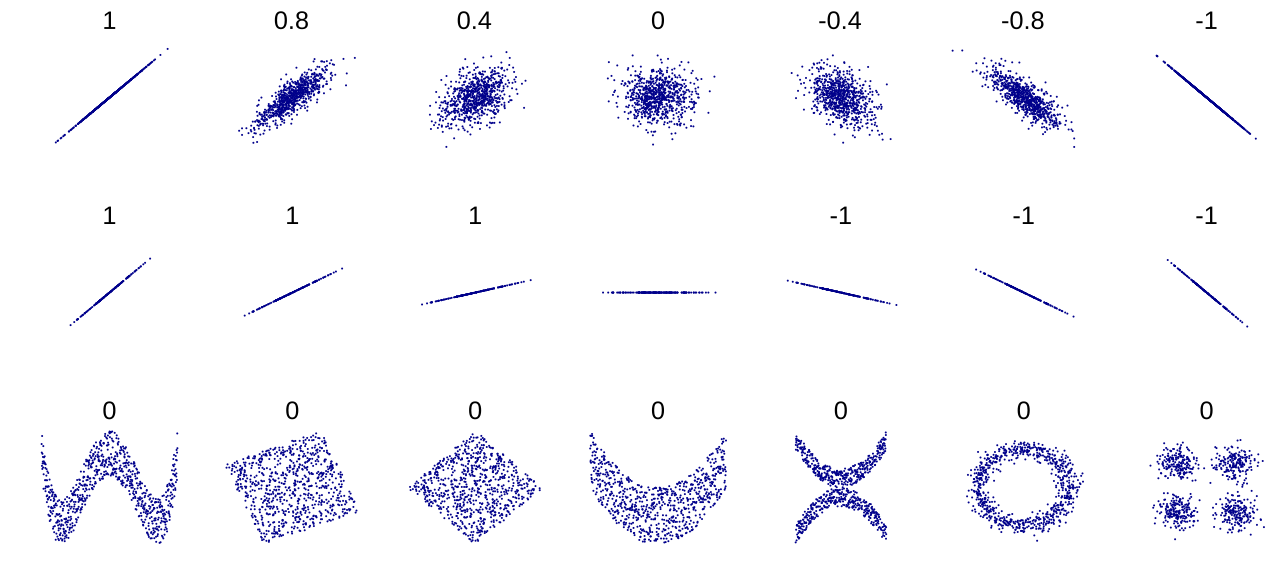
\includegraphics[width=1\linewidth]{figures_pedagogy/linear_corr.png}
    \caption{Some standard and some curious examples of measuring linear correlation between the horizontal and vertical axes.}
    \label{fig:pedagogy:linear_corr}
\end{figure}

\autoref{fig:pedagogy:linear_corr} demonstrates the limitations of the Pearson's correlation coefficient. The top row and center row show data with the same $r_{xy}$, but note how the noisier data in the top row can have identical $r_{xy}$ but look very different. The bottom row shows data with obvious correlation. That is, each data point is clearly related to each other. However, these datasets all have $r_{xy} = 0$

\subsection*{Probability}
Probability admits two primary interpretations, each with distinct philosophical and practical implications. \textbf{Frequentist probability} defines the probability of an event as its long-run relative frequency of occurrence:

\begin{equation}
    P(E) = \lim_{n \to \infty} \frac{\text{number of times E occurs}}{n}
\end{equation}

\noindent Under this view, after 101 coin flips yielding 51 heads, $P(\text{heads}) = 51/101 \approx 0.505$.

\textbf{Bayesian probability} treats probability as a degree of belief that can incorporate prior information. A Bayesian statistician who observes ten heads in a row but holds a strong prior belief that the coin is fair will still expect approximately $50\%$ heads in the long run. Conversely, if you were in the streets of Vegas and someone invited you to gamble on the outcome of a coin flip \textit{with their own coin}, you would not be likely to accept the bet, even if they flipped the coin a couple of times and got heads and tails once each. This flexibility makes Bayesian methods particularly powerful when data are scarce or when prior knowledge exists (for example, from theory, or from historical data about the same phenomenon).

For most introductory data exploration tasks, the frequentist interpretation suffices. However, many popular machine learning methods (\eg{} Gaussian processes, MCMC, Bayesian neural networks) explicitly rely on Bayesian reasoning.

\subsection*{Probability Arithmetic}
Probability obeys several fundamental rules. \textit{The} most fundamental rule being: probability is always represented by a number between 0 and 1 (which can alternately be represented by a number between $0\%$ and $100\%$). Furthermore, statisticians like to consider the concept of an `event,' and we like to give these events simple labels like `Event $A$' and `Event $B$.' Event $A$ may represent a coin landing heads up, and Event $B$ may represent a dice landing on a six. Mathematically, we represent the probability of such an event like so: $P(A)$ or $P(B)$. With this notation, we can now represent our first rule of probability like so: $0 \leq P(A) \leq 1$.

If Event $A$ is a coin landing heads up, we may also consider Event $\bar{A}$ where the coin lands tails up. $\bar{A}$ is said to be the \textit{complement} of $A$ and ― assuming the coin cannot land in any other state besides heads up or tails up ― $P(A) + P(\bar{A}) = 1$.

\subsubsection*{Independent (Disjoint) Events}
When two events are independent --- the two events do not influence each other whatsoever ― there exists a relationship between the probabilities of the two events. The mathematical way to state this is: $P(A) \cap P(B) = 0$ (where $\cap$ means 'intersection'). The probability of $A$ \textit{or} $B$ occurring, $P (A \cup B) $ (where $\cup$ means 'union'), is the sum of their probabilities. The probability of both $A$ \textit{and} $B$ occurring, $P (A \cap B) $, is the product of their probabilities. The \textbf{conditional probability} of $A$ given $B$, $ P(A|B)$, is the probability of Event $A$ happening given that Event $B$ has happened. For disjoint events, this is equal to $P(A)$ since $A$ and $B$ are independent.

The arithmetic rules for events with independent probabilities are:

\begin{align}
    \textrm{If }P(A) \cap P(B) = 0 \textrm{ then:}\\
    P(A \cup B) &= P(A) + P(B) \\
    P(A \cap B) &= P(A) * P(B) \\
    P(A | B) &= P(A)
\end{align}

\subsubsection*{Dependent Events}
When events are dependent upon each other in some way, the preceding rules no longer hold, and new relationships emerge. We may state a dependent relationship like so: $P(A) \cap P(B) > 0$. Consider the conditional probability $P(A|B)$ again. This quantity will now always be less than $P(A)$. Two more, less intuitive relationships emerge, which are stated below.

\begin{align}
    \textrm{If }P(A) \cap P(B) > 0 \textrm{ then:}\\
    P(A | B) &< P(A) \\
    P(A | B) &= \frac{P(A \cap B)}{P(B)} \\
    P(A \cap B) &= P(A) P(B|A)
\end{align}

\subsection*{Practical Data Exploration with Pandas}
In Python, the \verb`pandas` library provides the \verb`DataFrame` object, the workhorse for tabular data exploration. We will use the function \verb`pd.read_csv` to ingest a \verb`.csv` file and load it as a \verb`DataFrame` object. The \verb`DataFrame` object, often called \verb`df`, has many attributes and methods that are valuable for data exploration.

\begin{itemize}
    \item \verb|df.shape|: Returns (rows, columns). \textbf{Knowing the dimensionality of your data is paramount.}
    \item \verb|df.head(n)| and \verb|df.tail(n)|: Display first and last \verb|n| rows. This can reveal data entry errors, inconsistencies, or unexpected formatting.
    \item \verb|df.columns|: Lists all column names. This is the spine of your data. All analysis flows from knowing your columns (\textit{aka} `features').
    \item \verb|df.info()|: Provides column names, non-null counts, and data types. Missing data often appears here first, but only if the missing data is represented by null values (\verb|None| or \verb|nan|).
    \item \verb|df.describe()|: Generates summary statistics (count, mean, standard deviation, min, quartiles, max) for numeric columns. Pay particular attention to min/max values as they often expose outliers or coding errors.
\end{itemize}

\clearpage
\section{Statistics}
\subsection*{Learning Questions}
\begin{itemize}
    \item What is a distribution?
    \item What is a `moment' of a distribution?
    \item What can the quantiles of a distribution tell us?
    \item What is the Law of Large Numbers?
    \item What is the Central Limit Theorem?
\end{itemize}

\subsection*{Introduction}
Data in the real world (\ie{}, data not generated for the purpose of learning) emerge as observations drawn from underlying \textit{distributions.} Lesson 2 introduced probability as a framework for mathematical reasoning with random processes, and this lesson will teach the essential machinery of statistical distributions. Understanding these distributions, and their parameters and properties is necessary for most analyses.

We will discuss two important distributions: the Poisson and the Gaussian. The former is defined for discrete data, while the latter is defined for continuous data. I present these two distributions \textit{together} because, in a sense, they are cousins. In certain regimes, one can approximate the other. I present these two distributions \textit{first} because they enable us to understand the two most important ideas in statistics: The \textbf{Law of Large Numbers} and \textbf{The Central Limit Theorem.}

\subsection*{The Poisson Distribution}
The best way to form an intuitive understanding of any distribution is to examine an example that resonates with you. Since I don't know who \textit{you} are, I will choose an example that resonates with me.

Consider a leaky faucet. Every so often, a drop of water will form and drip from the faucet. As a statistician, you measure the rate of dripping over a long time and find that an average of two drops form every minute. However, you note that the number of drops per minute is a random variable; sometimes there are more drops, and sometimes there are fewer. You then might wonder: what is the probability that 4 drops form in one minute? The Poisson distribution comes to your rescue!

The Poisson distribution models the number of events occurring in a fixed interval of time (or space), given that events occur independently at a constant average rate (a \textit{stationary process}). We can define its \textbf{probability mass function} (PMF) as:

\begin{equation}
    P(X = k) = \frac{\lambda^k e^{-\lambda}}{k!}, \quad k = 0, 1, 2, \ldots
\end{equation}

The random variable --- the \textit{event} --- is $X$ and represents the number of drops that occur in a particular minute. We don't know what $X$ is, but we know that it is distributed according to a Poisson distribution with an average value, $\lambda$, of 2. The values that any distribution is defined on (\ie{} all the possible values that the phenomenon could take) are known as the \textbf{support}, and in the case of the Poisson distribution, we like to call it $k$. Since in this case $k$ measures a number of events, it cannot take negative or fractional values: the support of a Poisson distribution is non-negative integers, or $\mathbb{N}_0$.

With this meagre amount of knowledge of distributions, we can already answer our question about the leaky faucet. We know that $\lambda=2 \text{ drops per minute}$, and we want to know the probability of $k=4 \text{ drops}$ forming in one minute. Using the PMF:
\begin{equation}
    P(X=4) = \frac{2^4 e^{-2}}{4!} = 0.09
\end{equation}

There's a $\approx9\%$ chance of observing four drops in one minute from the leaky faucet. Wow! We can formalize the answer to our question with the statement: ``The probability of measuring $k$ drops in the time interval is $P(X=k)$.'' We can even state it more generally: ``The probability that the random variable $X$ takes on the value $k$ is $P(k)$.''

The Poisson distribution is a \textit{discrete} distribution; notice how $k$ can only be zero or a positive integer. You can only have a discrete number of drops after all. What if you had a random variable that takes on any real value?

\begin{figure}
    \centering
    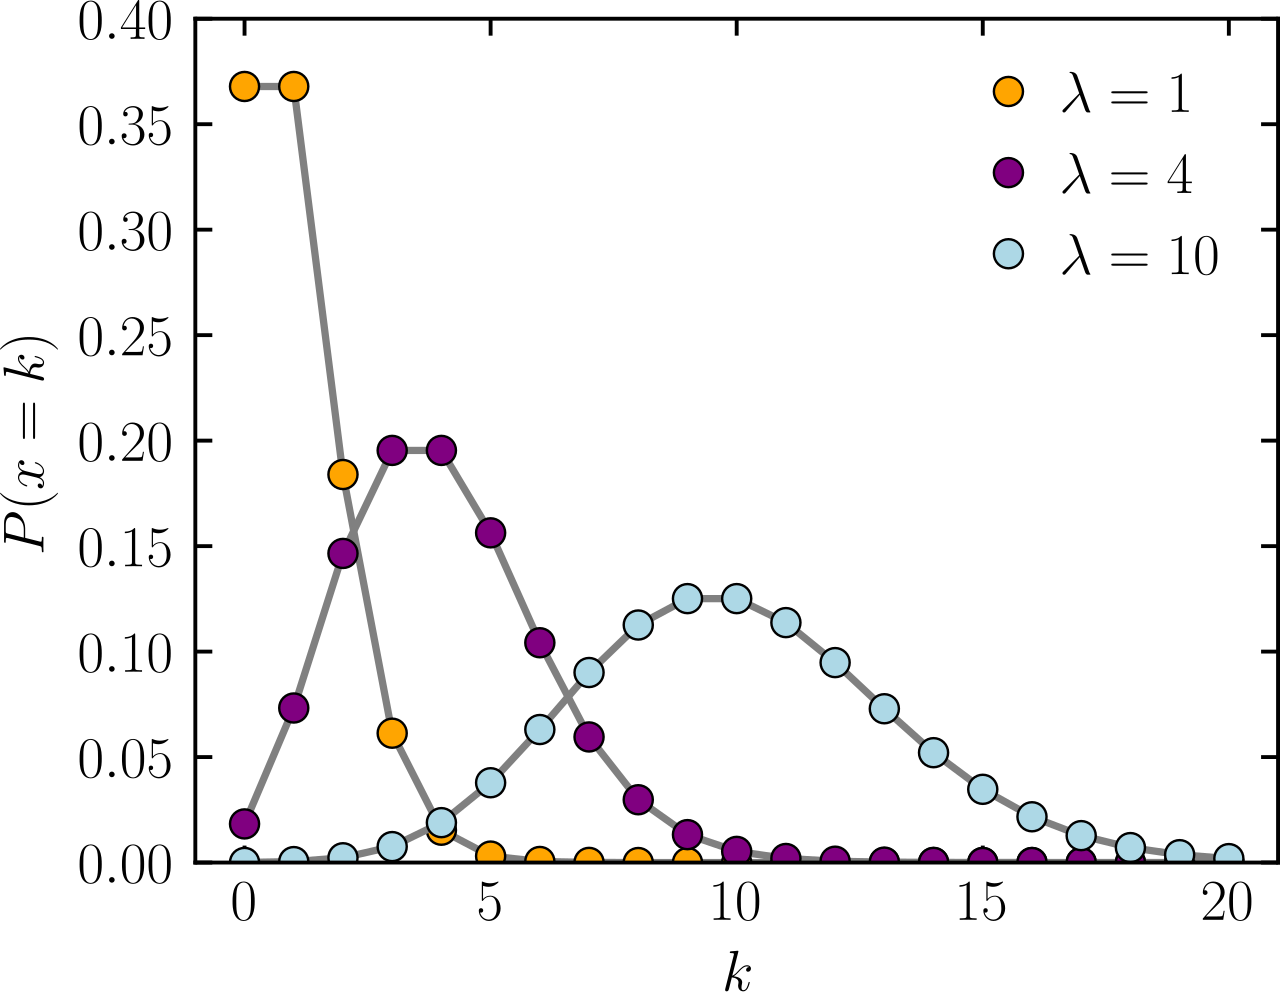
\includegraphics[width=1\linewidth]{figures_pedagogy/Poisson_pmf.svg.png}
    \caption{A plot of the probability mass functions for the Poisson distribution at three different values of $\lambda$. Image credit: Skbkekas (Wikipedia)}
    \label{fig:poisson_pmf}
\end{figure}

\subsection*{The Gaussian Distribution}
Consider a class of 100 students who take a test. To be accurate with our example, we must also imagine that the score of the test can take any real value between $0\%$ and $100\%$. The average result of their scores turns out to be $85\%$. Nice! Assuming that the scores are distributed according to a Gaussian (or Normal) distribution, what is the probability that a student scored between $80\%$ and $90\%$?

The Gaussian distribution is defined on a continuous support: all real numbers. Its \textbf{probability density function} (PDF) is:

\begin{equation}
    f(x;\mu, \sigma) = \frac{1}{\sigma\sqrt{2\pi}} e^{-\frac{1}{2}\left(\frac{x - \mu}{\sigma}\right)^2}, \quad x \in \mathbb{R}
\end{equation}

Where a Poisson distribution was defined by one number, the mean $\lambda$, the Gaussian is defined by two numbers: the mean $\mu$ and the standard deviation $\sigma$. A mathematical introduction to the standard deviation of a distribution will come in the next section, but for now, it is enough to say that the standard deviation defines how likely you are to measure the random variable far away from the mean. A small standard deviation means that the random variable is likely to be measured close to the mean, while a large standard deviation implies the opposite. Our class had a mean of $\mu = 85\%$ and a standard deviation of $\sigma = 5\%$. That means that not only did the students do well on average, but also the students mostly scored around $85\%$.

\begin{figure}
    \centering
    
\includegraphics[width=1\linewidth]{figures_pedagogy/gaussian_pdf.pdf}
    \caption{Two examples of a Gaussian probability distribution function with different means and standard deviations.}
    \label{fig:gaussian}
\end{figure}

There are a few things to note about the Gaussian distribution and our particular choice of example. First, our example has limited support. That is, $x$ can only take on values between $0\%$ and $100\%$. Gaussian distributions are defined on an infinite support (\ie{} $x$ can be any value between negative infinity and infinity; the mathematical way to say that is $x \in \mathbb{R}$), so technically what we have here is called a \textbf{truncated normal distribution.} For the purposes of this example, though, the differences aren't relevant (especially because with a small $\sigma$ the probability of getting values $<0\%$ or $>100\%$ is very low in our example, $<0.3\%$)               . 

Also note how we asked different types of questions in the leaky faucet example and the test example. In the former, we asked, ``What is the probability of observing \textit{exactly} four drops in one minute?'' And in the latter we asked, ``What is the probability that a student scored \textit{between} an $80\%$ and a $90\%$?'' For a discrete distribution, its probability \textit{mass} function (PMF) $P(k)$ gives the direct probability of observing exactly $k$. 

But if the support is continuous, as in the case of a Gaussian distribution, there are infinitely many values the function could take in any given interval of that support. So we can only define the probability $P(X \pm dx)$ of a continuous distribution as the probability the variable will take a value within a range $dx$, which can be as small or large as we want. We can, for example (and this will be important in the next lecture), ask what is $P(X \geq 0.05)$ or $P(X \leq 0.05)$.

It's also important to discuss special cases of the Gaussian/Normal distribution where $\mu=0$ and $\sigma=1$. We give this distribution a specific name: the \textbf{Standard} Normal Distribution, and a specific symbol for its PMF: $P_\mathcal{N}$. In this special case, $$P_\mathcal{N}(X \geq -1)  + P_\mathcal{N}(X \leq 1) = 68.2\%$$ and $$P_\mathcal{N}(X \geq -2) + P_\mathcal{N}(X \leq 2) = 95.4\%$$ In the next section we will see why, and in the next lecture, we will leverage this fact to test a hypotheses.

\subsection*{Moments of a Distribution}
Let's define something called a \textbf{moment} of some function, $f(x)$.

\begin{equation}
    \mu_n = \int^{\infty}_{-\infty} (x-c)^n\ f(x)\ dx
\end{equation}

\noindent where $f(x)$ is the function we are taking a moment of and $n$ is the ordinality of the moment (\ie{} first moment, second moment, third moment, etc.). In this instance, we would say ``$\mu_n$ is the $n$-th moment of $f(x)$ \textit{with respect to} $c$.'' When $c=0$, the moment is said to be a \textbf{raw moment.} The first raw moment of a distribution is the mean!

\begin{equation}
    \mu \equiv \mu_1 = \int^{\infty}_{-\infty} x\ f(x)\ dx
\end{equation}

When $c=\mu$ the moment is said to be a \textbf{central moment.} The first central moment is 0 by definition (it's not immediately obvious, but plugging in $c=\mu$ and $n=1$ to the moment equation and then simplifying will eventually yield 0), but the second central moment is something we call the \textbf{variance.} And it turns out that the variance is the square of what we called the standard deviation, $\sigma$. Isn't that neat!

\begin{equation}
    \sigma^2 \equiv \int^{\infty}_{-\infty} (x-\mu)^2\ f(x)\ dx
\end{equation}

The variance (and by extension the standard deviation) quantifies the \textit{spread} of the distribution, as we discussed before. There are two more moments worth discussing, the third and the fourth central moments.

The third central moment is called \textbf{skewness} and is a measure of the asymmetry of the distribution. The Gaussian is symmetric and thus it has 0 skewness. I encourage you to substitute the Gaussian into the moment equation with $c=\mu$ and $n=3$ to see this for yourself.

The fourth central moment is called \textbf{kurtosis} and is a measure of the \textit{tailedness} of the distribution. A distribution with positive kurtosis will appear to ``lean'' to the right, and a distribution with negative kurtosis will appear to ``lean'' to the left. Once again, you will find that the kurtosis of a Gaussian is 0. Overall, we can say that the moments of a distribution quantify its shape.

\subsection*{Quantiles and the Empirical Rule}
Quantiles divide a distribution into equal-sized intervals. For the Gaussian distribution, quantiles corresponding to integer multiples of the standard deviation are particularly important. \autoref{fig:stddevs} shows a standard normal distribution where each standard deviation from the mean is marked. The area under the curve in each of the regions is written above.

\begin{figure}
    \centering
    
\includegraphics[width=1\linewidth]{figures_pedagogy/stddevs.pdf}
    \caption{A standard normal distribution ($\mu=0$, $\sigma=1$). Each standard deviation is marked with vertical dashed lines and the percentage of the area under the curve in each region is annotated.}
    \label{fig:stddevs}
\end{figure}

Remember our test example? We said that $\mu=85\%$ and $\sigma=5\%$. Using this chart --- \textit{and assuming that the test scores are indeed distributed according to a Gaussian} --- we can say that $\approx 68\%$ of students will have scored within one standard deviation of the mean (between $80\%$ and $90\%$) and $\approx 95\%$ of students will have scored within two standard deviations (between $75\%$ and $95\%$).

\noindent \textbf{NB:} This concept will become exceptionally relevant in the next lecture on Null Hypothesis Rejection Testing.

\subsection*{The Law of Large Numbers}
Let's first define some terms: in statistics, we refer to a finite group of examples of a given phenomenon that you can collect data on (\eg{} a finite number of people you have access to for which you can measure, say, the height) as a \textbf{sample}. The entirety of the instances of that phenomenon in existence (the heights of everyone in the world, in this case) is a \textbf{population}.

Imagine you were trying to measure the average human height. At first you might have access to only two friends: your \textbf{sample size,} $n$, would be $2$ and your \textbf{sample mean,} $\bar{X}_n$ would be fairly inaccurate as a representation of the average human height since it only includes two samples. If you expanded your sample size then your sample mean would become more accurate --- it would become closer to the \textit{true} average human height. We would call this true average human height the \textbf{population mean,} $\mu$.

\textbf{The Law of Large Numbers} states that as the sample size increases, the sample mean converges to the population mean. This convergence explains the intuitive knowledge that larger samples will yield more stable estimates.

\subsection*{The Central Limit Theorem}
The Central Limit Theorem (CLT) is arguably the most important result in introductory statistics. It's important to internalize --- this will come with time and practice --- but it's most important for its implication for scientific measurements. To understand the CLT, consider the following scenario. Let the set $\{X_1, X_2, ..., X_N\}$ be a random sample of size $N$ from some population. And let the distribution (it can be any\footnote{It cannot be \textit{any} distribution but you'll learn the exceptions as they come up.} distribution) of that population have mean $\mu$ and variance $\sigma^2$. Let the mean of the sample be $\bar{X}_N$. The CLT then states that $\bar{X}_N$ is a random variable described by a Gaussian distribution with mean $\mu$ and variance $\sigma^2/N$.

\textbf{Read that again.} It's ok, I'll wait.

The implications of this should not be immediately obvious to you, but consider this scenario: a scientist is attempting to measure some value. It doesn't matter what the value is; maybe it's the average rate of the dripping faucet from before. If the scientist were to take $N$ different measurements of the average rate of the dripping faucet (this would be $\{X_1, X_2, ..., X_N\}$ representing the number of drops that fell in time intervals $\{t_1, t_2, ..., t_N\}$), then the CLT tells the scientist the average value of those measurements will be distributed according to a Gaussian. And not just any Gaussian! A Gaussian whose mean \textit{is} the true value of the rate of the dripping faucet. Not to mention, the CLT also tells us about the variance --- the shape --- of the underlying distribution.

Measuring the rate of a dripping faucet may not be very interesting, but many sciences boil down to the measurement of variables. The CLT gives us the    confidence that we can measure these variables and place limits on how well we know them.

\clearpage
\section{Null Hypothesis Rejection Testing}
\subsection*{Learning Questions}
\begin{itemize}
    \item What is the principle of falsifiability?
    \item What is Null Hypothesis Rejection Testing (NHRT)?
    \item Why do we use NHRT?
    \item What is the Z-test?
    \item What is a one-tailed test? What is a two-tailed test?
    \item What is a p-value?
    \item What is a statistic?
    \item What is p-hacking?
    \item What is the KS-Test?
\end{itemize}

\subsection*{Introduction}
The most basic formalism of science can be hastily distilled into one sentence: test an idea with data. That sentence does a lot of heavy lifting. Testing an idea with data is hard! One question naturally arises: How do we know when data supports an idea and when it does not? This is where \textbf{Null Hypothesis Rejection Testing} (NHRT) comes in.

NHRT is based on the \textbf{Principle of Falsifiability} formulated by philosopher Karl Popper in 1934 in \textit{The Logic of Scientific Discovery.}  An idea --- formally called a \textbf{hypothesis} --- must be falsifiable. Whatever your hypothesis is, it must be logically \textit{and practically} possible to contradict it. The canonical example of a falsifiable hypothesis is: ``All swans are white.'' Simply observing one swan that is not white is enough to falsify this hypothesis.

\subsection*{The NHRT Algorithm}
Let's construct an example to demonstrate how we test hypotheses. Consider a Bus that takes some route, Route $A$. The total trip duration of Route $A$ is known to follow a Gaussian distribution with a mean of $\mu = 34 \text{ min}$ and a standard deviation of $\sigma=2.4 \text{ min}$. One day, the Bus company alters the bus route in order to shorten travel times. Let's call the new bus route, Route $B$. The bus company measured the total trip duration for Route $B$ 100 times. Does this $N=100$ sample provide enough evidence to conclude that Route $B$ is faster than Route $A$?

\subsubsection*{Step 1: Formulate The Prediction}
We start by constructing a \textbf{null hypothesis} ($H_0$). This must be a falsifiable statement that represents something we seek to falsify. A null hypothesis that states ``The world is not round,'' would imply that our belief is that the world \textit{is} round and that we seek to show evidence for it. ``The coin is fair,'' would imply that we are trying to show that the coin is not fair. For our bus example we might say that ``Route $B$ produces the same trip durations as Route $A$.'' But we can get more specific.

\begin{quote}
    $H_0$: The sample of Route $B$ trip durations comes from a population with $\mu_0 = 34 \text{ min}$.
\end{quote}

\noindent Our goal with NHRT is to analyze our evidence and determine if we can \textit{falsify} the premise set forth by the null hypothesis.

\subsubsection*{Step 2: Identify All Alternative Outcomes}
Next we construct the \textbf{alternative hypothesis} ($H_1$), which is the logical complement of the null hypothesis. If $H_0$ is ``The world is not round,'' then $H_1$ would be ``The world is round.'' If $H_0$ is ``The coin is fair,'' then $H_1$ would be ``The coin is not fair.'' Notice how the combination of $H_0$ and $H_1$ encompasses every single logical possibility (conversely, \eg{} ``The world is flat'' would not complement ``The world is not round,'' correctly, as it leaves out infinite other possible shapes). In our case, the appropriate alternative hypothesis would be ``Route $B$ produces different trip durations than Route $A$.''

There is a small hiccup here. We are actually interested in knowing whether Route $B$ produces \textit{shorter} trip durations than Route $A$. What we're interested in the \textbf{single-tailed} alternative (as opposed to a \textbf{double-tailed} one, where Route $B$ is simply a different duration, longer or shorter):
\begin{quote}
    $H_1$: The sample of Route $B$ trip durations comes from a population with $\mu_0 < 34 \text{ min}$.
\end{quote}

\noindent $H_1$ is not strictly the complement of $H_0$ because it's a single-tailed alternative, but that's alright. However, this choice of directionality has important consequences for the test, as we will see.

\subsubsection*{Step 3: Set a Confidence Threshold}
The scientist must determine how much evidence they require in order to reject the null hypothesis. We set this threshold of evidence by stating a confidence level, $\alpha$, which represents the probability of rejecting $H_0$ \textit{when it's actually true.} This is known as a Type I error. Colloquially, you could say ``There is an $\alpha\%$  probability that the evidence indicates we should reject the null hypothesis when the null hypothesis is actually true.''

Once more: we must determine for ourselves how much evidence we need to reject the null hypothesis. No one else will do it for us. The way we do this is by selecting a confidence threshold \textit{before} we perform the rest of the NHRT algorithm. This threshold represents the probability that the data indicates to us (through the use of the forthcoming statistical test) that we should reject the null hypothesis even though, in reality, it's true.

For the null hypothesis of ``The world is round,'' we might choose $\alpha=0.01$. This means we are asserting that there is a $1\%$ chance that the world is indeed round even though our data suggests otherwise. How can we possibly know what value of $\alpha$ to use? We don't. We don't set the confidence threshold by estimating it. We set it by \textit{deciding} how rigorous we want our test to be. Choosing a very small threshold and then rejecting the null hypothesis indicates high confidence in the outcome of the test. You can set a large threshold, but the validity of your result will be less potent. There are standards on this in different fields. For example, in the social sciences, it is common to choose $\alpha=0.05$, since social sciences deal with human behavior, and humans are complex. In particle physics, conversely, the standard is $3\times10^{-7}$ (0.0000003). In other words, if a particle physicist were to repeat their experiment 3.5 million times, only one of those times would the data ``trick'' the physicist, and encourage them to reject the null hypothesis when it's actually true.

Let's choose $\alpha=0.05$ for this example.

\subsubsection*{Step 4: Find a Pivotal Quantity with a Known Distribution Under $H_0$}
A \textbf{pivotal quantity} (or test statistic) is a function of the data whose probability distribution is known when $H_0$ is true. For our example, we will choose the \textbf{Z-statistic}:

\begin{equation}
    Z = \frac{\bar{X} - \mu_0}{\sigma_0 / \sqrt{n}}
\end{equation}

\noindent where $\bar{X}$ is the sample mean, $n$ is the sample size and $\mu_0$ and $\sigma_0$ are the \textit{population} mean and standard deviation under $H_0$ (\ie{} $\mu_0=34\text{ min}$ $\sigma_0=2.4\text{ min}$). By the Central Limit Theorem (CLT), we know that when $n$ is sufficiently large, the sampling distribution of $\bar{X}$ is approximately normal, and consequently $Z$ follows a standard normal distribution with mean 0 and standard deviation 1, or in mathematical notation, $Z \sim P_\mathcal{N}$.

But if $Z$ is a number extracted from a standard normal distribution, from the previous lecture, we \textit{know} what the probability of getting a number \textit{as large} or \textit{as small} as $Z$, because we know the PMF $P_\mathcal{N}$. For example, if $Z$ is extracted from a Gaussian distribution with mean $\mu=0$ and standard deviation $\sigma=1$, and $Z>1$, we would know that the probability of getting $Z>1$ is $P(Z>1) = (100-68)/2 = 16$\% (see \autoref{fig:stddevs})!

\subsubsection*{Step 5: Calculate the Pivotal Quantity}
Imagine that we calculate $\bar{X}$, which is the average of the 100 Route $B$ trip durations and find that $\bar{X}=34.46\text{ min}$. We then compute the Z-statistic:

\begin{equation}
    Z = \frac{34.46 - 34}{2.4 / \sqrt{100}} = 1.94
\end{equation}

The Z-statistic tells us that the sample mean of Route $B$ trip durations lies 1.94 standard deviations *above* the population mean of $\mu_0$. That is to say that the Route $B$ trip durations are longer than the Route $A$ trip durations. Not good. But let's see if the statistic says this is significant compared to our confidence threshold.

\subsubsection*{Step 6: Test the Data Against Alternative Outcomes}
The \textbf{p-value}, $p$, is the probability, under the null hypothesis, of obtaining a test statistic at least as extreme as the one observed. That is, the p-value is $P(Z>1.94)$ if $H_0$ is true. And keep in mind that $H_0$ being true implies that our statistic is distributed according to a standard normal distribution $Z \sim P_\mathcal{N}$. Crucially, the p-value is *not* the probability that $H_0$ is true.

\begin{equation}
    p = 2 \Phi(| Z |) = 0.052 \equiv 5.2\%
\end{equation}

I've introduced a new symbol here, $\Phi$, the \textbf{Cumulative Distribution Function} (CDF) of the standard normal distribution. I'll come back to what the CDF is and how we calculated the p-value, but let's first accept this value as correct and figure out what it means for our null hypothesis.

In fact, let's remind ourselves what our null and alternative hypotheses were. $H_0$: ``The sample of Route $B$ trip durations comes from a population with $\mu_0 = 34 \text{ min}$.'' $H_1$: ``The sample of Route $B$ trip durations comes from a population with $\mu_0 < 34 \text{ min}$.''

The p-value is saying: ``There is a $5.2$\% probability that one would observe our sample of Route $B$ trip durations while $H_0$ is true.'' In other words, this p-value is telling us that there is a $5.2$\% probability of observing these trip durations even though Route $B$ is the same as Route $A$. This doesn't address whether Route $B$ is shorter or longer, just whether it's different. We chose a p-value threshold of $5$\%, and our calculated p-value is \textit{not} smaller than our threshold. This means that we \textit{cannot} reject the null hypothesis.

There are two misconceptions we should talk about. First, the p-value is not the probability that the null hypothesis is true. It is the probability of observing data at least as extreme as what we did observe while assuming the null is true. Second, failing to reject $H_0$ is not the same as accepting $H_0$. Absence of evidence is not evidence of absence; our sample may be too small to detect a small effect.

\subsubsection*{The Cumulative Distribution Function}
The CDF is the integral of the PDF along the support or, in simpler terms, the CDF is the area beneath the PDF curve. So if you imagine the bell-shaped curve of the standard normal distribution (\autoref{fig:stddevs}), the CDF at some point $x$, $\Phi(x)$, is the area between the bell curve and the $x$-axis between $-\infty$ and $x$. In integral form, it looks like this:

\begin{equation}
    \Phi(x) = \int_{-\infty}^{x} f(x') dx'
\end{equation}

\noindent where $f(x)$ is the PDF and $x'$ is a dummy variable for integration.

\begin{figure}
    \centering
    
\includegraphics[width=1\linewidth]{figures_pedagogy/gaussian_cdf.pdf}
    \caption{Two cumulative distribution functions of a Gaussian distribution with different mean and standard deviation. See \autoref{fig:gaussian} for the corresponding PDFs.}
    \label{fig:cdf}
\end{figure}

What does the CDF tell us? The CDF evaluated at some point, $x$, is the probability that our random process will take on a value that is less than or equal to $x$. Relating this back to the bus routes example, we can learn some things. We already know that our $Z\text{-statistic}$ is distributed according to a standard normal distribution, which, by definition, has a mean of $0$. We calculated that $Z=1.94$. What is the probability that $Z$ could be either $\geq 1.94$ or $\leq -1.94$? In other words, what is the probability that $Z$ is at least as extreme as what we calculated? This is the $p\text{-value}$!

\clearpage
\section{Introduction To Machine Learning}
\subsection*{Learning Questions}
\begin{itemize}
    \item What is data?
    \item What is machine learning?
    \item What is a model?
    \item What is the difference between a parameter and a hyperparameter?
    \item What is the difference between supervised and unsupervised learning?
    \item What is an objective function?
    \item What is Ordinary Least Squares (OLS) regression?
    \item How do we evaluate model performance?
    \item Why do we split data into training, validation, and test sets?
    \item What is overfitting?
\end{itemize}

\subsection*{Introduction}
Imagine you are trying to teach a computer to recognize handwritten digits. You could try to write explicit rules: ``A seven has a horizontal line across the top and a vertical line on the right.'' But what about different handwriting styles? What about smudges? What about a seven written with a serif? You would spend forever writing rules, and your program would still fail on the first handwritten note you gave it. There must be a better way.

And there is! Instead of programming the rules explicitly, you can show the computer many examples of handwritten digits and let it discover the rules itself. This is \textbf{supervised machine learning.}

\subsection*{Part 1: What Is Data?}
Before we can build models, we must understand the types of data we work with. The NOIR taxonomy classifies data into four levels of measurement. Each level supports different mathematical operations, and using the wrong operation on the wrong type of data leads to nonsense.


\begin{table}
    \centering
    \begin{tabular}{c|cccccc}
         & Order & Distance & Mean & Median & Mode & Absolute Zero \\ \hline
        Nominal & x &  &  & x & & \\
        Ordinal & x &  &  & x & x & \\
        Interval & x & x & x & x & x & \\
        Ratio & x & x & x & x & x & x\\
    \end{tabular}
    \caption{NOIR data. The four types of data and their features.}
    \label{tab:noir}
\end{table}

\textbf{Nominal data} consist of unordered categories. Colors are nominal. Bus route numbers are nominal. You can't say one color is ``more'' than another; you cannot calculate the average of $\{\text{blue}, \text{green}, \text{orange}\}$. The mode --- the most frequently occurring category --- is the only appropriate measure of central tendency.

\textbf{Ordinal data} have order but not equal spacing. Movie ratings (1–5 stars) are ordinal. You know that 5 stars is better than 1 star, but you cannot claim that a 4-star movie is ``twice as good'' as a 2-star movie. The difference between 4 stars and 5 stars may not mean the same thing as the difference between 1 star and 2 stars. The median and mode are appropriate, but the mean is not.

\textbf{Interval data} have equal spacing but no true zero. Temperature in Celsius or Fahrenheit is interval. Twenty degrees Celsius is hotter than ten degrees Celsius, and the ten-degree difference means the same thing anywhere on the scale. However, twenty degrees Celsius is \textit{not} twice as hot as ten degrees Celsius because zero degrees Celsius doesn't represent an absence of temperature. The mean, median, and mode are all meaningful.

\textbf{Ratio data} have equal spacing \textit{and} a true zero. Temperature in Kelvins is ratio. Twenty Kelvins \textit{is} twice as hot as ten Kelvins. Zero Kelvins represents absolute zero, the complete absence of thermal energy.\footnote{Any system at $0\text{ K}$ would still have some zero-point energy, so this statement isn't completely true.} All arithmetic operations, including ratios, are valid.

\noindent \textbf{NB:} Many introductory data science projects treat all numeric data as ratio data. This is a mistake. If your data lacks a true zero, reporting that ``the average temperature doubled'' is mathematically incorrect.

\subsection*{Part 2: What Is Machine Learning?}
One time in 1959, some important guy\footnote{Arthur Samuel, a pioneer in machine learning.} said something really insightful about machine learning. ``[Machine learning is] the field of study that gives computers the ability to learn without being explicitly programmed.'' This... is not a very helpful definition for us. But it's poetic! And it will serve us for now. Let's go over some important terms.

A \textbf{model} is a low-dimensional representation of a higher-dimensional dataset. Consider a scatter plot of 100 points that roughly follow a straight line. The raw data contains 100 x-values and 100 y-values; that's 200 numbers. But a linear fit can be described by just two numbers: the slope and the intercept. That is a model: it is a simplification that captures the essential pattern while discarding the noise.

\textbf{Parameters} are learned from the data. In the linear model $y = mx + b$, the slope $m$ and intercept $b$ are parameters. The learning algorithm adjusts them to fit the training data.

\textbf{Hyperparameters} are set by you before training begins. They represent a decision that you have made about how you want your model to be. They are not learned from the data. You must choose them based on your own knowledge.

\subsection*{Machine Learning Paradigms}
Machine learning can be done in all sorts of different ways. To explain them, we first need to understand the concept of a \textbf{feature.} If you are recording the name, height and age of your friends, then `name,' `height' and `age' are the features of your dataset. They're also often called `columns' because data is often stored in a 2D, tabular format where each row represents one \textbf{object} (one of your friends) and each column contains one feature (\eg{} name, height and age).

Sometimes we use machine learning to predict one feature based on other features. This is called \textbf{supervised learning.} For example, you could try to predict someone's age based on their name and height. Or you could try to predict their name based on their height and age. Both of those sound like practically impossible tasks, but you could try it! The two main types of supervised machine learning are \textbf{classification,} where the goal is to predict (classify) a nominal or ordinal feature, and \textbf{regression} where the goal is to predict (regress) an interval or ratio feature.

Supervised learning is probably the most common type of machine learning, but \textbf{unsupervised learning} is almost as ubiquitous. In this paradigm, you aren't trying to predict one of your features. Rather, you are looking for structure within the features. The commonest applications are: \textbf{clustering,} partitioning data into groups of similar points; \textbf{anomaly detection,} identifying unusual observations that do not fit the pattern; \textbf{dimensionality reduction,} compressing data while preserving important information.

All of the tasks we will cover in this course will be supervised and unsupervised learning, but there are other paradigms worth mentioning. \textbf{Semi-supervised learning} combines a small amount of labeled data with a large amount of unlabeled data. This is common when labeling is expensive, but unlabeled data is abundant. \textbf{Active learning} allows a model to interactively query the user for labels on particularly informative data points. The model asks: ``What is \textit{this} one?'' and you tell it. With \textbf{reinforcement learning,} the model (agent) learns to make sequential decisions by maximizing a cumulative reward signal through interactions with an environment.\footnote{Reinforcement learning is really cool! Maybe I will add a lesson on it one day.}

\subsection*{Part 3: Model Fitting and Objective Functions}
For now, we will focus on supervised machine learning where our ultimate goal is to use our features to predict some target by fitting a model. Fitting a model involves two steps.

\textbf{Step 1:} Choose a mathematical form. Do you have a reason to believe that there is an underlying linear relationship between your feature and your target? You could visualize your data and decide for yourself what model to use too, but keep in mind that this introduces biases. It's best to pick a model based on your theoretical understanding of the data. But, for a linear relationship, you might choose the model $y = mx + b$.

\begin{figure}[t]
    \centering
    
\includegraphics[width=0.5\linewidth]{figures_pedagogy/linearmodel.pdf}
    \caption{A collection of data points spread out in a rough line is approximated by a linear model. In this case, the parameters of the model are $m=1$ and $b=0$.}
    \label{fig:linearmodel}
\end{figure}

\textbf{Step 2:} Optimize an \textbf{objective function} (also called a loss function) that quantifies how well the model fits the data. Consider the machine learning task posed in \autoref{fig:linearmodel} where we have a collection of data points, and we want to fit a linear model to it. We don't know what the parameters of the model are yet (that's what machine learning does), so we're going to guess the parameters first and then see how good that guess was. In order to evaluate how good the guess is, we will use this objective function that compares the predictions of the model with our guessed parameters to the true target values. Then, the objective function returns one number which lets us know if the parameters were good or not.

The \textbf{sum of absolute errors} (SAE), also called the L1, is one such objective function:

\begin{equation}
    L_1 = \sum_{i=1}^n |y_i - \hat{y}_i|
\end{equation}

\noindent where $n$ is the number of samples/objects/rows in your data, $y_i$ is the $i$-th target, and $\hat{y}_i$ is the model's prediction of $y_i$. Thus the ``error'' that is being summed is $|y_i - \hat{y}_i|$. Notice that when $y_i$ and $\hat{y}_i$ are close to each other (when the prediction of the model is good and errors are low), then $L_1$ is small.

The \textbf{sum of squared errors} (SSE), or L2, is another objective function:

\begin{equation}
    L_2 = \sum_{i=1}^n (y_i - \hat{y}_i)^2
\end{equation}

\noindent The difference here is that the L2 squares the error rather than summing them together. What this means practically is that when the errors are large (\ie{} $|y_i-\hat{y}_i|>1$) then $L_2$ is always larger than $L_1$.

These two objective functions are the most primitive and most useful for teaching and learning, but they're certainly not the best. In fact, there is no ``best'' objective function. You always want to choose the objective function that is best for your machine learning task; in this way, the choice of the objective function is a hyperparameter.

\subsubsection*{Ordinary Least Squares (OLS) Regression}
Depending on your choice of objective function, you may be able to analytically solve for the best parameters (\ie{} do some clever math rather than guessing and checking). If you have some data, and you want to model it with a line, and you want to use the L2 objective function, then there happens to be such an analytic solution for the parameters $m$ and $b$ based on the data. Neat!

\begin{align}
    m &= \frac{\sum_{i=1}^{N} (x_i - \bar{x})(y_i - \bar{y})}{\sum_{i=1}^{N} (x_i - \bar{x})^2} \\
    b &= \bar{y} - m\bar{x}
\end{align}

\noindent where $\bar{x}$ and $\bar{y}$ are the average values of $x$ and $y$ in your data.\footnote{You may have encountered this before under a different name. When I was in high school, I learned about the ``line of best fit,'' which was almost certainly the OLS method.}

\subsection*{Part 4: Model Performance Metrics}
We already discussed how the objective function quantifies how good of a model you have, but we can generalize that idea further. A \textbf{metric} is any function that measures how good a model is. The distinction between the metric and the objective function is that the objective function may not mean anything to a human. If you calculated the L2 for a dataset and a model and found $L_2 = 1.5$, what would you do with that information? You could try to wrap your head around it, but for the most part, objective functions are only useful in comparison. If you changed the model parameters and found $L_2=1.4$, then you could say that the model improved because the L2 decreased. A metric is \textit{generally} somewhat easier to understand.

\begin{align}
    \epsilon_i &= y_i - \hat{y}_i \quad \text{(Error)} \\
    SAE &= \sum_i^n |\epsilon_i| \quad \text{(L1 or Sum of Absolute Errors)} \\
    SSE &= \sum_i^n \epsilon_i^2 \quad \text{(L2 or Sum of Squared Errors)} \\
    MAE &= \frac{1}{n} \sum_i^n |\epsilon_i| \quad \text{(Mean Absolute Error)} \\
    MSE &= \frac{1}{n} \sum_i^n \epsilon_i^2 \quad \text{(Mean Squared Error)} \\
    RMSE &= \sqrt{MSE} \quad \text{(Root Mean Square Error)}
\end{align}

\noindent I've introduced three new metrics (they can also be used as objective functions): the \textbf{mean absolute error,} the \textbf{mean squared error} and the \textbf{root mean square error.} The first two are simply the L1/SAE and L2/SSE divided by the number of samples. This makes the quantity a bit simpler to understand. All of these are commonly used, but there is one more that is ubiquitous in linear modeling: the \textbf{coefficient of determination} or simply the ``R-squared.''

\begin{align}
    RSS &= \sum_i^n (y_i - \hat{y}_i)^2 \quad \text{(L1 or SAE or ``Residual Sum of Squares'')} \\
    TSS &= \sum_i^n (y_i - \bar{y})^2 \quad \text{(``Total Sum of Squares'')} \\
    R^2 &= 1 - \frac{RSS}{TSS} \quad \text{(Coefficient of Determination)}
\end{align}

Unfortunately it's true that the \textbf{residual sum of squares} (RSS), L1 and SAE are all the same thing, but I've re-written it here for clarity because I've also introduced the \textbf{total sum of squares} (TSS) where the sum is not over the errors but over the difference between $y_i$ and the $\bar{y}$, the mean. The $R^2$ is always between 0 and 1, where a ``perfect'' model is a 1, and a model that always predicts $\bar{y}$ would be a 0. What the $R^2$ actually measures is the proportion of variance in $y$ that is \textit{explained} by the model. A model with $R^2=0$ predicts only the mean, and it doesn't account for any of the variance from the mean within the data. A model with $R^2=1$ perfectly predicts every single variation from the mean.

For classification problems, the metrics and objective functions are entirely different. The objective functions are necessarily less simple because math with discrete variables is unusual for most of us. We will just cover four common classification metrics for now.

Let's say we are predicting a target based on some data. The target we are predicting has two possibilities: positive or negative. Whenever we make a prediction, there are four possibilities: we predict positive and the target was positive (a \textbf{true positive,} TP); we predict negative and the target was negative (a \textbf{true negative,} TN); we predict positive and the target was negative (a \textbf{false positive,} FP); we predict negative and the target was positive (a \textbf{false negative,} FN). Table~\ref{tab:confusion_table} represents these four outcomes in \textbf{confusion matrix.}

\begin{table}
    \centering
    \begin{tabular}{c|c|c}
                      & Prediction is $+$ & Prediction is $-$ \\ \hline
        Target is $+$ & TP               & FN \\ \hline
        Target is $-$ & FP               & TN \\
    \end{tabular}
    \caption{An example ``confusion matrix'' demonstrating the four possible outcomes of binary classification.}
    \label{tab:confusion_table}
\end{table}

We can now define our four metrics based on those four outcomes:

\begin{align}
    \text{Accuracy} &= \frac{TP + TN}{TP + FP + TN + FN} \\
    \text{Precision} &= \frac{TP}{TP + FP} \\
    \text{Recall} &= \frac{TP}{TP + FN} \\
    F_1 &= \frac{2TP}{2TP + FP + FN}
\end{align}

\noindent \textbf{Accuracy} is simply the proportion of correct predictions. \textbf{Precision}\footnote{also called positive predictive value (PPV)} is the fraction of true positives to all of the positives that the model predicted. Precision answers the question: ``How many retrieved items are relevant?'' \textbf{Recall}\footnote{also called sensitivity} is the fraction of true positives among all positives. Recall answers the question ``How many relevant items are retrieved?'' Finally, we have the \textbf{F1-score}, which is actually the harmonic mean of Precision and Recall, therefore representing both equally within one metric. All four of these metrics can take on values between 0 and 1, and can therefore be represented by percentages.

\subsection*{The Split: Training, Validation, and Test}
Here is a trap that ensnares many students: You fit a model to your data and you evaluate its performance on that data. The performance looks great, you find $R^2 = 0.95$ (regression) or $F_1=99\%$ (classification). Then you come across some new data, and you try your model on it and find the metrics have plummeted. What happened?

Your model learned the data it trained on, including its noise and quirks. It did not learn the underlying pattern. This is called \textbf{overfitting;} the model was not generalizable. To honestly assess generalizability, you must split your dataset into three non-overlapping subsets. The \textbf{training set}, \textbf{validation set} and \textbf{test set.}

The training set is where the model learns its parameters. For example, if you were to use the OLS method to find the parameters of a linear model, you would calculate $\bar{y}$ and $\bar{x}$ on this training set. The validation set is used to tune hyperparameters. You evaluate performance here repeatedly, though you don't train on it. Perhaps you want to know what the effect of changing the objective function would be? You would compare the two models' performance on the validation set. Lastly, the test set is used \textit{only once,} ever, at the very end of your project. When you write your research paper on your cool new model, in the results z you will include the performance of the model on this test set. You never use the test set to inform any model parameters or hyperparameters.

\subsubsection*{Overfitting and Underfitting}
When your model is too simple to capture the underlying pattern in the data, we say the model is underfitting. Imagine fitting a straight line to data that clearly follows a curve. Underfitting produces poor performance on both the training set and validation set. You could improve the model by changing hyperparameters (\eg{} going from a linear model to a quadratic model). Overfitting occurs when your model is too complex relative to your amount of data. The model learns noise and idiosyncrasies specific to the training set, and the fundamental pattern or physical system that created your data is lost. Overfitting produces excellent performance on the training set but poor performance on the validation set. The dataset split is your primary defense against overfitting.

While we learn the parameters from the data in the training set, we change the hyperparameters based on the performance of the validation set. We may choose a quadratic model instead of a linear one if we see the model underfitting on the validation set. Or we might choose a linear model instead of a quadratic one if we see overfitting. This is why splitting the data into two sets is not sufficient. We need a third test set to make sure the hyperparameters were not tuned specifically to the validation data. The theme here is that we want our models to generalize, and the only way to ensure that is to hide parts of the dataset from our model and then surprise it at the end.

\subsection*{Optimization}
We discussed objective functions, formulae that quantify how poorly or how well a model fits data. The L1 objective sums absolute errors. The L2 objective sums squared errors. Both return a single number: the error. The smaller the number, the better the model. But knowing the error is only half the problem. How do we find the model parameters that minimize the error? This is the task of \textbf{optimization.}

The simplest optimization method is brute force. You try every possible combination of parameters and compute the objective function for each, picking the parameters that lead to the smallest value. If your model has only one continuous parameter, that is actually \emph{infinite} values you have to calculate the loss for. You cannot do that, so where do you start? What is the first value you test? Perhaps you will choose 0 to be your starting point. Now what is the next point? 0.1? 0.01? The smaller this number, the more calculations you have to make and the more likely you ``step over'' the minimum. The issue with the brute force method is that there is no limit to how many parameters you'll need to test. We will use \textbf{gradient descent} instead.

Imagine you are standing in a mountainous landscape, blindfolded. Your goal is to find the lowest point. You can feel the slope beneath your feet, so if the ground slopes downhill to your left, you take a step to the left. If it then slopes downhill to your right, you take a step to the right. You could repeat this process until you can no longer feel any downward slope.

Optimization algorithms work the same way. The ``mountainous landscape'' is the \textbf{loss landscape}: a surface that maps model parameters to the value of the objective function. The ``lowest point'' in the loss landscape is the set of parameters that minimizes the objective function. The ``slope'' is the gradient of the loss landscape.

The gradient is like your feet: it can tell you what direction the landscape is sloping. Mathematically, it is the derivative of the loss at that value of the parameter vector. The gradient is a vector that points in the direction in which the loss landscape is steepest. We want to traverse down the loss landscape, so we calculate the gradient of the objective function and move in the opposite direction of the gradient. And when I say ``move'' I mean ``try a new set of parameters.'' In practice, we will try a set of parameters, calculate the objective function, calculate the gradient of the objective function at that point, and then change the parameters in the opposite direction (\ie{} increase or decrease each parameter) of the gradient.

Consider a simple objective function: a parabola, $f(x)=x^2$, where x is the model parameter. The minimum value that $f(x)$ takes on is at $x=0$, $f(0)=0$. But let's say we didn't know that (because in general, objective functions are more complicated), and start at $x=2$. The gradient (or just the derivative, for functions of one parameter) is $f'(x)=2x;f'(2)=4$. The gradient at $x=2$ is $4$; it's positive. Thus, we should decrease our parameter to move in the opposite direction of the gradient. Let's try $x=-2$. The gradient is $f'(x=-2)=-4$, negative, which means we should increase our parameter.

Once we have the gradient, we know whether to increase or decrease our parameters, but by how much? This \textbf{step size} is controlled by the \textbf{learning rate} hyperparameter. A small learning rate means you make small changes to your parameter in proportion to the gradient, and a big learning rate means you make big changes to the parameter in proportion to the gradient. Small learning rates mean your optimizer will be cautious and slow. Large learning rates mean your optimizer will be risky (you may overshoot the minimum), but fast. Choosing the right learning rate requires you to balance your desire for speed and algorithm stability.

Gradient descent works well, but it requires you to calculate the objective function on the entire training set at each step. \textbf{Stochastic gradient descent} (SGD) computes the gradient using only a single, randomly chosen (hence ``stochastic''), data point. The objective function evaluated on one data point may be wildly different compared to another, but this is actually a strength of SGD. The gradient is noisy and imprecise, but this helps with avoiding local minima.

A local minimum is a valley that is not the lowest point in the entire landscape. Standing in a local minimum, it would feel like you're at the lowest point, but perhaps over the nearby hill is an even deeper valley. You would never know, just by measuring the slope at your location. The noise in the calculated gradient can help kick the algorithm out of a local minimum. 

There is also \textbf{mini-batch gradient descent} where, instead of using the entire dataset (gradient descent) or a single point (SGD), mini-batch gradient descent uses a small random subset of the data to compute the gradient. This balances the accuracy of the gradient estimate (which improves with more points) with the ability to avoid local minima. Local minima are a significant challenge in optimization, especially for models with many parameters, so mini-batch gradient descent, or some variant of it, is very common.

\clearpage
\section{Regression and Classification}
\subsection*{Learning Questions}
\begin{itemize}
    \item What is multiple linear regression?
    \item What is logistic regression?
    \item Why is logistic regression ``classification?''
\end{itemize}

\subsection*{Introduction}
In the previous lesson, we covered machine learning as a whole, and we talked a lot about the linear model $y=mx+b$. If we have some feature $x$ and we have some target $y$, and we believe there is a linear relationship between them, then we can use the linear model to predict $y$ based on $x$. This is called \textbf{simple linear regression} because there is one feature, $x$. When there is more than one feature that we want to use in our model, but we still want the model to be linear (\ie{} we never exponentiate $x$), that is called \textbf{multiple linear regression} (also sometimes called \textit{multilinear} regression).

\subsection*{Regression: Multiple Linear Regression}
This lesson will formalize the simple linear regression we talked about last time with some new notation that we can more easily expand the concept to multiple linear regression. This lesson will make use of some simple vector and matrix arithmetic. To start with, we will now refer to our parameters as a vector $\boldsymbol{\beta}=[\beta_0,\beta_1,...,\beta_p]$. We will also refer to our set of observations --- our features and targets --- like so: $\{\mathbf{x}_i,y_i\}_{i=1}^n$, where the vector $\mathbf{x}_i=[x_{i1},x_{i2},...,x_{ip}]$ represents the observation of $p$ features for observation $i$.\footnote{I'm using the same notation that the Wikipedia page for ``Ordinary least squares'' uses, and I encourage you to look at that page for --- if nothing else --- an alternative wording of the same math which may help aid in your understanding.} We can also write our vector of targets as $\mathbf{y}=[y_1,y_2,...,y_n]$.

That's a lot of math. Let's give that a quick example because this is important and confusing. Imagine that we have a dataset of daily temperature, humidity and rainfall. Temperature and humidity are our features, and rainfall is our target.\footnote{Note that rainfall is also a feature, but we are choosing this feature to be the one that we predict based on the others.} We have two features, so $p=2$. Let's say that this data is recorded for three days, so $n=3$. For one observation, we have three numbers: temperature $T$, humidity $H$, and rainfall $R$. Using the same notation as before, let's write out our observations $\mathbf{x}_1$, $\mathbf{x}_2$ and $\mathbf{x}_3$.

\begin{align*}
    \mathbf{x}_1&=[T_1,H_1] \\
    \mathbf{x}_2&=[T_2,H_2] \\
    \mathbf{x}_3&=[T_3,H_3]
\end{align*}

\noindent We can compare this to our earlier notation to see that, when $i=1$, $x_{i1}=T_1$ and $x_{i2}=H_1$, and so on. Something useful we can do with this is rewrite our linear model in terms of vectors:

\begin{align*}
    y &= 
    \begin{bmatrix}
        1 & x
    \end{bmatrix}
    \cdot
    \begin{bmatrix}
        b \\
        m \\
    \end{bmatrix} \\
    y &= (1 \cdot b) + (x \cdot m) \\
    y &= b + mx
\end{align*}

\noindent All I did was rewrite $y=mx+b$ in terms of vectors and then simplify the expression to get back to $y=mx+b$ to prove to you they are identical. Now let's apply this same thing to our general notation. For each $y_i$, we can write our own linear equation with vectors:

\begin{align*}
    y_i &= 
    \begin{bmatrix}
        1 & T_i & H_i
    \end{bmatrix}
    \cdot
    \begin{bmatrix}
        \beta_0 \\
        \beta_1 \\
        \beta_2
    \end{bmatrix} \\
    y_i &= (1 \cdot \beta_0) +  (T_i \cdot \beta_1) + (H_i\cdot \beta_2)
\end{align*}

\noindent What we end up with is a simple equation. Do you notice how $b$ and $\beta_0$ aren't being multiplied by any feature? Just like $b$, $\beta_0$ is the \textit{intercept} of the equation, and you can think of $\beta_1$ as the \textit{slope for Temperature}, and $\beta_2$ as the \textit{slope for humidity}.

We can take all of this one step further and write down an equation not just for one target $y_i$, but for every target $\mathbf{y}$. To do this we need to define $\mathbf{X}$, the ``design matrix,'' ``model matrix'' or ``regressor matrix.''

\begin{equation}\label{eq:X}
    \mathbf{X} = 
    \begin{bmatrix}
        1 & T_1 & H_1 \\
        1 & T_2 & H_2 \\
        1 & T_3 & H_3
    \end{bmatrix}
\end{equation}

\noindent We can put all this together now in one beautiful equation:

\begin{align}
    \label{eq:linearmodel1}
    \mathbf{y} &= \mathbf{X} \boldsymbol{\beta} \\
    \label{eq:linearmodel2}
    \begin{bmatrix}
        y_1 \\
        y_2 \\
        y_3
    \end{bmatrix} &=
    \begin{bmatrix}
        1 & T_1 & H_1 \\
        1 & T_2 & H_2 \\
        1 & T_3 & H_3
    \end{bmatrix} \cdot
    \begin{bmatrix}
        \beta_0 \\
        \beta_1 \\
        \beta_2
    \end{bmatrix}
\end{align}

\noindent With great pleasure, allow me to introduce to you the \textbf{linear model} \autoref{eq:linearmodel1}. With this equation, we can now express a linear model for any number of features! This is the key to multiple linear regression. If you aren't familiar with linear algebra, it may not yet be clear how this is useful to us. I'm sure you agree that the equation is beautiful, but the whole point of machine learning is that we need to find those parameters, $\boldsymbol{\beta}$!

Let's rewrite the sum of squared errors (SSE) with our new notation.
\begin{align*}
    SSE_i &= \sum_{i=1}^n (y_i - \hat{y}_i)^2 \\
    SSE &= ||\mathbf{y}-\mathbf{X}\boldsymbol{\beta}||^2
\end{align*}
\noindent where the $\hat{y}_i=\mathbf{x_i}\cdot\boldsymbol{\beta}$ is the \textbf{estimator} for $y_i$. In other words, $y_i$ is the $i$-th observation of our target and $\hat{y}_i$ is what our model predicts for $y_i$.

There is an analytic solution for the best parameters $\boldsymbol{\beta}$, that minimize $SSE$. Just like the last lesson, this solution is called the ordinary least squares solution:

\begin{equation}\label{eq:ols}
    \boldsymbol{\beta} = (\mathbf{X}^\intercal \mathbf{X})^{-1} \mathbf{X}^\intercal \mathbf{y}
\end{equation}

\noindent We know $\mathbf{X}$, it's just the design matrix which is just our features from our data. We know $\mathbf{y}$, it's just the targets in our dataset. If you can construct $\mathbf{X}$ and $\mathbf{y}$, you can do multiple linear regression. Congratulations!

\subsubsection*{Notation}
Notice how I denote a vector with a bold lowercase letter (\eg{} $\mathbf{x}_i$, $\mathbf{y}$, $\boldsymbol{\beta}$), I delimit vectors with brackets (\eg{} $\boldsymbol{\beta}=[\beta_0,\beta_1,...,\beta_p]$, $\mathbf{x}_i=[x_{i1},x_{i2},...,x_{ip}]$, $\mathbf{y}=[y_1,y_2,...,y_n]$), I delimit sets with braces (\eg{} $\{\mathbf{x}_i,y_i\}_{i=1}^n$), and I denote matrices as bold capital letters (\eg{} $\mathbf{X}$ in \autoref{eq:X}). Something else to note is that $p=n+1$ always. In words: the number of parameters (for a linear model) is always equal to the number of features, plus one.

\subsection*{Classification: Logistic Regression}
That's a rather curious section title, isn't it? Is it classification or is it regression? Well, it's both! Let's return to our example data with temperature $T$, humidity $H$, and rainfall $R$. As it stands, temperature is interval data, humidity is measured as a fraction between 0 and 1 so it's ratio data, and rainfall is measured in some unit of length like inches so it's also ratio data. Let's change rainfall from ratio data to nominal data: did it rain or did it not rain? Our rainfall feature is now binary. How do you predict a binary variable?

Linear regression won't help us here. If you encode your data as zeros and ones, it is indeed possible to perform linear regression, but the model won't be very helpful. Most of the time it's going to end up predicting $0.5$ which is neither a $1$ or a $0$. We need another model.

\textbf{Logistic regression} is all about the logistic function in the same way that linear regression was all about the linear function. The logistic function (\autoref{fig:logistic}) has quite an unusual form, both mathematically and graphically:

\begin{equation}\label{eq:logistic}
    \sigma(x)=\frac{1}{1+e^{-x}}
\end{equation}

\begin{figure}
    \centering
    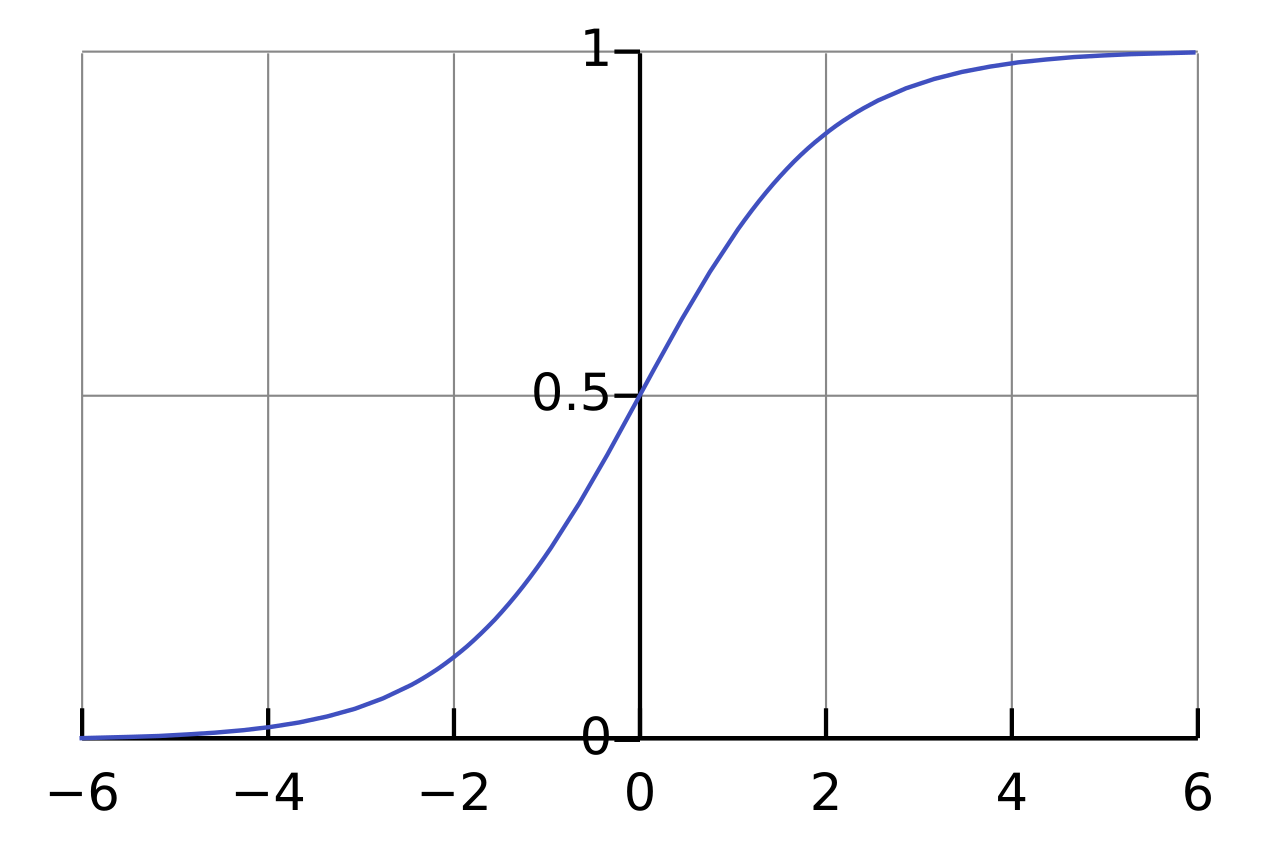
\includegraphics[width=0.5\linewidth]{figures_pedagogy/Logistic-curve.svg.png}
    \caption{The logistic function.}
    \label{fig:logistic}
\end{figure}

The logistic function takes any input and always produces an output between 0 and 1. Which, you may notice, is quite handy if you are trying to predict a binary variable. \autoref{eq:logistic} depicts the simplest version of the logistic function, but we can create a logistic model by introducing some parameters:

\begin{equation}
    p(x)=\frac{1}{1+e^{-(\beta_0 + \beta_1 \cdot x + \ldots)}}
\end{equation}
\noindent where the parameter vector $\boldsymbol{\beta}$ and the design matrix $\mathbf{X}$ makes a return.

We need an objective function for this new model so we can figure out what the best parameters are. We also need to choose a threshold for classification. Did you notice how in \autoref{fig:logistic}, the logistic function can output numbers between 0 and 1? This is not a problem: if the logistic model predicts a number $\geq0.5$, we count it as a 1, otherwise it's a 0.\footnote{You don't have to choose a threshold of $0.5$.} We are treating the output of the logistic model as a probabilistic classification.

You may wonder, how is this any different from the linear model if it also doesn't have a binary output? The linear model produces an output between $-\infty$ and $\infty$, whereas the logistic function produces an output between 0 and 1 no matter the input. Also, the graph of the logistic function as it transitions from outputting 0 to outputting 1 is a quick s-curve, whereas the linear model produces a straight line. These two things make it impossible to consider the output of the linear model a probabilistic classification, and this is why logistic \textit{regression} is actually classification.

\subsubsection*{The Logistic Loss Function}
The objective function we'll use is called the \textbf{logistic loss} or simply log loss.\footnote{The log loss is equivalent (up to a constant) to the cross-entropy loss, which is used in neural networks.}

\begin{equation}\label{eq:logloss}
    \ell = \sum_{i=1}^n (y_i \ln(p_i) + (1-y_i)\ln(1-p_i))
\end{equation}

\noindent where $\ell$ is the log loss, $n$ is the number of observations, $y_i$ is the $i$-th target (0 or 1), and $p_i$ is the probabilistic classification from the logistic model (between 0 and 1).

Unfortunately, there is no analytic solution like there is for the linear model; I cannot write an equation that starts with $\boldsymbol{\beta}=$, which is spiritually devastating. Must we determine $\boldsymbol{\beta}$ by ``brute force''? Checking every combination of our parameters until we find a good result? In the last lesson we discussed optimization schemes, so no. But for now, yes, we will find our parameters by brute force.\footnote{Strange as it is, brute force is the \emph{technical} term for computing all possible solutions (in a range) to choose the best one.}

\subsubsection*{Nominal Features}
What if you have a feature in your dataset that is nominal? Imagine that you have a dataset and one of the features is titled ``Blood Type.'' You look through the dataset, and you find that there are only four different entries in this feature: A, B, AB, and O. This is certainly nominal data, but most people would call this a categorical variable. How do we turn categorical variables into something that we can do math with?

The answer is a process called \textbf{one-hot encoding.} We expand the ``Blood Type'' feature into four different features: ``Blood Type: A,'' ``Blood Type: B,'' ``Blood Type: AB,'' and ``Blood Type: O.'' In each of these four new features, we input a 1 in the corresponding column. \autoref{tab:onehot} shows what this would look like in a tabular dataset.

\begin{table}
    \centering
    \begin{tabular}{c|cccc}
        Blood Type & Blood Type: A & Blood Type: B & Blood Type: AB & Blood Type: O \\ \hline
        A  & 1 & 0 & 0 & 0 \\
        B  & 0 & 1 & 0 & 0 \\
        AB & 0 & 0 & 1 & 0 \\
        O  & 0 & 0 & 0 & 1 \\
    \end{tabular}
    \caption{An example of one-hot encoding.}
    \label{tab:onehot}
\end{table}

\subsubsection*{Min-Max Normalization}
Min-max normalization is a simple process that scales all numeric features to the range $[0, 1]$:

\begin{equation}
    x_{\text{scaled}} = \frac{x - x_{\text{min}}}{x_{\text{max}} - x_{\text{min}}}
\end{equation}

Why is this necessary? Consider two features: income (ranging from \$0 to \$200,000) and age (ranging from 0 to 100). Income has a much larger scale. Without normalization, income would dominate the model and age would contribute almost nothing. Normalization puts all features on equal footing.

\subsection*{More on the Split: Training, Validation and Test}
In the last lesson we touched on why you want to split your data into three non-overlapping subsets: the training set, the validation set and the test set. But I did not provide any guidance on how much you should allocate for each set. After all, you only have one dataset. It's not easy to get more data; we work with what we have. If you have $100$ observations, you need to figure out how many go into each set.

The training set is where the model learns its parameters. You want this set to be as large as possible. A larger training set gives the model more examples to learn from, which usually leads to better generalization. Every data point you hold back for validation or testing is one the model cannot learn from.

The validation set is where you monitor performance during training. You use it to tune hyperparameters, compare different models, and detect overfitting. You want this set to be as large as possible too. A larger validation set gives you a more reliable estimate of how the model is performing. If your validation set is too small, random noise can mislead you. A dip in validation accuracy might just be bad luck, not overfitting. A spike might be good luck, not genuine improvement.

The test set is where you prove that your model works. You use it exactly once, at the very end of your project, to report final performance. You want this set to be as large as possible as well. A larger test set gives you a more trustworthy final evaluation. If your testing set is too small, you cannot be confident that your model will perform well on new data.

So if we want all three sets to be as large as possible, what do we do? Allocate a third of the data to each set? There is no perfect ratio that works for every situation. A massive dataset with millions of rows can afford to hold out $20\%$ for validation and $20\%$ for testing while still leaving plenty for training. A tiny dataset with only 100 rows cannot afford to hold out anything.

The most important thing is not the specific ratio you choose, it's that \textbf{each set is representative of the population your data comes from.}

Let's consider an example. Imagine you are building a model to predict housing prices. Your data contains houses from five different cities. If you put all the houses from City A into the training set and all the houses from City B into the test set, your evaluation will be meaningless. The model will learn the patterns specific to City A, and you will test it on a completely different distribution of houses. Your test set performance will tell you nothing about how the model would perform on a new house from City A or C.

The splits must preserve the underlying structure of your data. If your data has categories, each split should contain a representative proportion of those categories. If your data comes from different time periods, each split should span the same range of time. In practice, you achieve this by using \verb|train_test_split| from the \texttt{sci-kit learn} package with appropriate arguments: \verb|stratify| for categorical targets, \verb|shuffle| to randomize order, and \verb|random_state| to make your results reproducible.

So, maybe you are reading this section because you just want to know what size your sets should be. Unfortunately, I truly can't tell you. There is no single correct answer. You must consider your total sample size, the complexity of your problem, the noise in your data and the cost of making a mistake. If you were to read this section and conclude that the best \textit{starting place} is a one-third split for each set, that is fine. But never forget: \textbf{the representativeness of your splits matters more than the exact ratios.}

\clearpage
\section{Tree Models}
\subsection*{Learning Questions}
\begin{itemize}
    \item What is a decision tree?
    \item What is Gini impurity?
    \item What are the hyperparameters of tree models?
    \item What are ensemble methods?
    \item How does regression with tree models work?
\end{itemize}

\subsection*{Introduction}
Decision trees are among the most intuitive and interpretable types of machine learning models. They mimic the way humans make decisions: by asking a series of questions, each of which narrows down the possibilities until a conclusion is reached. But despite their simplicity, decision trees are also among the most successful types of models, seeing widespread use in all disciplines.

\subsection*{The Decision Tree}\label{sec:pedagogy:trees}
A decision tree is a kind of flowchart, where each internal node represents a test --- a question --- on a feature. Each branch of the tree represents the outcome of the test, and each leaf represents the output of the model (a classification or a regression). To make a prediction, you start with your observation you want to predict on, $\mathbf{x}_i$, and you traverse the tree by answering questions about your observation until you reach a leaf.

\autoref{fig:dtc} provides an example of a decision tree classifier. The dataset has three features: outlook (sunny, rain), humidity ($0-100\%$), and windy (yes, no). The target variable is whether or not a sports game will be allowed to be played (play, don't play). We read the decision tree from the root node at the top (it's an inverted tree). The first node asks ``What is the outlook?'' Outlook is a categorical variable with two categories. A branch spawns for each possible answer to the question: one if the outlook is `sunny,' and one if it's `rain.' Within the node, you'll notice that, among all of the observations that could traverse the tree and arrive at that node, the amount of observations with the target variable `play,' or `don't play,' is written. 

\begin{figure}
    \centering
    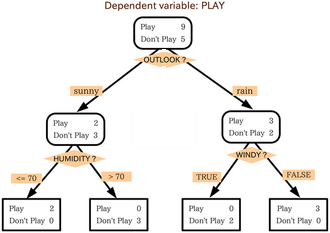
\includegraphics[width=0.5\linewidth]{figures_pedagogy/Decision_tree_model.png}
    \caption{An example decision tree.}
    \label{fig:dtc}
\end{figure}

Along the bottom layer, we actually see that all four of the leaf nodes (remember that a node with no branches is called a leaf) have either only `play' or only `don't play.' We call this a pure node. Compare this to the node at the end of the `sunny' branch, which is not pure.

You may be wondering: how does the model know which question to ask at each node? The goal of the model is to ask a question that leads to the purest nodes. To do this, we need a way to quantify node purity.

\subsection*{Gini Impurity}
The \textbf{Gini impurity} is a common metric for measuring the purity of a decision in a tree. If the dataset has $J$ class labels ($J=2$, `play' and `don't play'), the Gini impurity can be written as: 

\begin{align}
    G &= 1 - \sum_{i=1}^{J} p_i^2 \\
    J=2 \quad G &= 1 - (p_1^2 + p_2^2)
\end{align}

\noindent where $p_1$ is the relative frequency of class label 1 (`play') and $p_2$ is the relative frequency of class label 2 (`don't play')  (they are denoted as $p$ because, as we discussed in \autoref{sec:pedagogy:stats}, frequencies \emph{can} be interpreted as probabilities, unless you work in a Bayesian framework).

Let's calculate the impurity of some of the nodes in \autoref{fig:dtc}. Consider the root node, where the total number of samples is $N=N_1+N_2=9+5=14$. The relative frequency of `play' is $N_1/N=64\%$, and for `don't play' it's $N_2/N=36\%$. To calculate the Gini impurity:

\begin{align*}
    G &= 1 - (p_1^2 + p_2^2) \\
    G &= 1 - \left( \left(\frac{N_1}{N}\right)^2 + \left(\frac{N_2}{N}\right)^2 \right) \\
    G &= 1 - \left( 0.64^2 + 0.36^2 \right) \\
    G &= 46\%
\end{align*}

\noindent Now that we have some practice calculating the Gini impurity on the root node, let's do it for each of the three nodes after the root node.

\begin{align*}
    \text{sunny} \quad G &= 1 - \left( \left(\frac{2}{5}\right)^2 + \left(\frac{3}{5}\right)^2 \right) = 48\% \\
    \text{rain} \quad G &= 1 - \left( \left(\frac{3}{5}\right)^2 + \left(\frac{2}{5}\right)^2 \right) = 48\% \\
\end{align*}

\noindent If we look at all of the four leaf nodes on the bottom, they will all have a Gini impurity of $0\%$. They are minimally impure, or in other words, they are maximally pure!

As a final test, let's imagine we have a new sample (\ie{} a day to schedule a game) in our dataset and we want to use our model to predict the target. The new sample has the following feature values: outlook rain, humidity $80\%$, windy yes. The first node we travel down is the `rain' branch to the `windy' node. Then we travel down the `True' branch to the final leaf node. The final prediction is therefore the class label most represented in the leaf node; in this case, the final prediction is `don't play'.

What happens if the target variable remains mixed at the leaf node? There is no guarantee that you can achieve purity. It is possible that under the same conditions, you get two different outcomes. If the leaf node is not pure, the prediction can be the most common label in that leaf, or it can be interpreted as a probability: if a leaf node contained 3 `don't play' and one `play' labels the prediction for a day that falls in that leaf node would be a 75\% ``probability'' of no game (we put ``probability'' in quotes because it is not a probability in a Bayesian sense, which is what we most often want to achieve with machine learn models).

\subsubsection*{Decision Trees and Data Types}
Decision trees can handle both categorical and numerical features. For categorical or numerical features alike, a question at a node \textit{always} splits the data into two branches. In \autoref{fig:dtc}, one node question is whether the humidity is $\leq70\%$ or $>70\%$. This threshold is chosen to minimize the Gini impurity. 

\subsubsection*{Decision Tree Hyperparameters}
Decision trees have several important hyperparameters that govern their growth and complexity. Here I refer specifically to the \verb|scikit-learn| implementation of decision trees.

\verb|max_depth|: The maximum depth of the tree. This isn't how many branches can be made; it's how many rounds of decisions can be made. In \autoref{fig:dtc}, the total depth was two. Deeper trees can capture more complex patterns but are more prone to overfitting. With an unlimited number of trees, the model \textit{will} overfit.

\verb|min_samples_split|: The minimum number of samples required to split an internal node. Higher values prevent the tree from making splits on very small subsets, which, again, reduces overfitting.

\verb|min_samples_leaf|: The minimum number of samples required to be at a leaf node. This ensures that leaf nodes always represent a meaningful number of observations.

\verb|max_features|: The number of features to consider when looking for the best split. Restricting the number of features can introduce randomness, which is beneficial for ensemble methods (which we will discuss later in this lesson).

\verb|criterion|: There are different ways to measure the quality of a split apart from Gini impurity. Entropy is the other common criterion you will see.

\subsubsection*{Pruning}
Decision trees are notorious for overfitting. A tree that is allowed to grow until every leaf is pure will perfectly classify the training data, but perform poorly on unseen data. The model will have learned every single intricacy of the training set, including the noise, but its generalizability will be very poor.

Overfitting occurs because the tree can continue splitting until each leaf contains samples of only one class. This is particularly problematic when the dataset is small relative to the number of features, like in \autoref{fig:dtc}. Several techniques can prevent overfitting in decision trees. The simplest is \textbf{early stopping:} halting the growth of the tree when certain criteria are met, such as reaching a maximum depth or a minimum number of samples per leaf. \textbf{Pruning} is another approach where the tree is first grown to its full size. Nodes that do not provide significant improvement in predictive power are then removed.

\subsection*{Ensemble Methods}
While a single decision tree is easy to visualize and understand (something we call ``interpretability''), its predictive power is often limited. Ensemble methods address this by combining multiple trees to produce a more robust prediction. The underlying principle is that a collection of not-so-good decision trees (called ``weak learners'') that are only slightly better than a random guess can form a good decision tree (``strong learner'') when combined appropriately.

\subsubsection*{Random Forests}
A \textbf{random forest} is an ensemble of decision trees, each trained on a random bootstrap sample\footnote{A sample drawn with replacement from the dataset. That is: select a subset of size $N$ out of a dataset of size $M$, where $N < M$; do that several times, each time selecting $N$ from the full $M$ objects, and treat each subset separately.} of the data. This means that each tree sees a slightly different set of training examples. Additionally, at each split, the tree only considers a random subset of the features. In our previous example, this would mean that one of the weak learners ignores humidity while the other ignores outlook. These two quirks help ensure that the trees are not correlated with each other.

When making a prediction, each tree in the figurative forest ``votes'' for a class (the majority class in that leaf node for that tree), and the class with the most votes is provided by the model as the official prediction. The philosophy is that, while some trees may be misled by noise in their training data, the majority vote of many trees will converge on the correct answer. Random forests are more robust to overfitting than single decision trees. 

\subsubsection*{Gradient Boosting}
\textbf{Gradient boosting} is another ensemble tree method. Instead of building trees in parallel to each other, gradient boosting builds trees sequentially. Each new tree is trained to correct the errors made by the previous trees. The algorithm fits a tree to the residuals (the difference between the true class and the predicted class), then adds this tree to the ensemble.

Gradient boosting is particularly powerful for complex classification problems. The \verb|XGBoost| library is an optimized implementation of gradient boosting that also includes other features like regularization, which we will discuss more thoroughly in the lesson on neural networks.

\subsubsection*{Boosting and Bagging}
Two terms you hear often in machine learning spaces are \textbf{boosting} and \textbf{bagging.} Bagging (bootstrap aggregating) is used in random forests. Trees are built independently, trained on bootstrap samples, and the final prediction is an average of all of the trees. Boosting is used in gradient boosting; trees are built sequentially. Each tree focuses on the mistakes of the previous ones. Bagging helps to curtail overfitting, while boosting helps to reduce model bias. Both types of models are useful. In fact, you may want to try both on the same task to see which is best.

\subsubsection*{Regression}
The decision tree algorithm seems naturally inclined towards classification tasks; however, it is equally capable of regression. A \textbf{regression tree} predicts a continuous variable instead of a class. Instead of Gini impurity, regression trees use a splitting criterion based on the reduction in MSE of the target variable.

\subsection*{Interpretability}
Decision trees are remarkably interpretable. A trained tree can be visualized and understood by anyone. This interpretability is a major advantage in contexts where understanding the relationship between the features and the target is as important as making accurate predictions. However, decision trees are prone to instability. Small changes in the training data can lead to vastly different splits and thus vastly different trees. The order of the splits matters. Ensemble methods mitigate this instability.

\subsection*{Feature importance}
Tree models provide a measure of \textbf{feature importance.} By tracking how much each feature reduces impurity across all splits in a tree, we can determine which features are the most important for prediction. In a Random Forest, we can also obtain a measure of the variance of the importance by looking at the variance of its impact for all splits across different trees. 

\clearpage
\section{Clustering}
\subsection*{Learning Questions}
\begin{itemize}
    \item What is clustering?
    \item What is the $k$-means algorithm?
    \item Why is feature scaling important for clustering?
    \item What is DBSCAN?
    \item What is hierarchical clustering?
    \item What is a dendrogram?
    \item What are the different types of clustering good at?
\end{itemize}
\subsection*{Introduction}
Imagine that you are a school administrator. You have data on students: their attendance percentage and their homework scores. You want to find out if there are ways to group these students based on their attendance and homework scores. You don't have anything to predict, no labels or features to regress; you just want to know if there is some structure in your data. This is the problem of \textbf{clustering.} Clustering is an unsupervised learning method. Unlike classification or regression, where we have information that we want to learn how to predict, clustering finds structure within unlabeled data. It partitions data points into groups (clusters) such that points within the same cluster are similar to each other, and points in different clusters are dissimilar.

In this lesson, we will cover three major clustering methods: $k$-means, DBSCAN and agglomerative clustering. Before we begin, recall the four types of data: NOIR. Clustering requires a definition of similarity or distance between data points. As a result, clustering is most appropriate for interval and ratio data, where distances are meaningful. Clustering on nominal or ordinal data requires special care (\ie{} a more abstract definition of distance).

\subsection*{$k$-means Clustering}
$k$-means is the most intuitive clustering algorithm. The goal is to partition our data into $k$ clusters. Each cluster is represented by its \textbf{centroid} --- the mean of all points in the cluster. The algorithm assigns each point to the cluster whose centroid is closest. In our student example, we have two features: attendance and homework score. Each student is a point in this 2D feature space, \ie{} each student can be represented by a point $(a,b)$ where $a$ is their participation and $b$ is their homework score (the same way a place is identified by two coordinates, \eg{} longitude and latitude). Let's say we suspect the students' attendance and scores are grouped based on who their teacher is. Three teachers teach a different section of physics, so we're going to try to group our data into three clusters, $k=3$. The $k$-means algorithm will find three centroids and assign each student to the nearest one. The result is that each student can now be represented by three points: $(a,b,c)$ where $c$ is one of the three clusters. We guessed that the students have different attendances and homework scores based on their teacher, so we would expect to see all students from one class belong to the same cluster. Having just taken random guesses for the coordinates ($\mu_a,\mu_b$) of each center, we are likely not there yet.

$K$-means minimizes the \textbf{inertia}.
\begin{equation}
    \sum_{i=1}^{k} \sum_{\mathbf{x} \in C_i} (\mathbf{x} - \boldsymbol{\mu}_i)^2
\end{equation}
\noindent where $\mathbf{x}$ is a point in the feature space (in our example it's a 2D vector), $C_i$ is the set of points in cluster $i$, and $\boldsymbol{\mu}_i$ is the centroid of cluster $i$ (also a 2D vector). The expression $(\mathbf{x} - \boldsymbol{\mu}_i)^2$ is the square of the Euclidean distance between two points, and in 2D space it can be expanded to $(a-a_{\mu_i})^2 + (b-b_{\mu_i})^2$.

In words: for each cluster, we compute the distance from each point to the cluster centroid. We square that distance, and sum all of them up. Then we sum them for each cluster. The goal of the algorithm is to minimize the inertia by choosing $\mu_i$'s appropriately.

\subsubsection*{The Algorithm}
The $k$-means algorithm has four steps.

\begin{enumerate}
    \item Initialize the locations of the $k$ centroids randomly in the feature space.
    \item Assign each point to the nearest centroid.
    \item Update each centroid to the mean of its assigned points.
    \item Repeat the last two steps until the location of the centroids stops changing.\footnote{In practice, this would be a very risky stopping condition because there may be unstable configurations where points swap back and forth from the clusters. What we actually use is ``repeat until the inertia does not change by more than a chosen threshold''.}
\end{enumerate}

It may be that the initial locations of the centroids were not optimal, resulting in centroids that aren't well placed. This is the risk we take with algorithms that have random elements. You can initialize the centers yourself if you like, but it's also common to run the algorithm many times with different starting points, and choose the result with the lowest inertia.

\subsubsection*{The Elbow Method}
How do we choose $k$? In our example, we chose it based on our knowledge of the context of the data. This is always the best way to pick any hyperparameter like $k$. But what if our data is too abstract, or very high dimensional, and there is no real way to understand the context? The \textbf{elbow method} is one way to choose $k$. 

\begin{figure}
    \centering
    
\includegraphics[width=0.5\linewidth]{figures/elbowMethod.png}
    \caption{A visualization of the ``elbow'' method to choose the number of clusters in $k$-means clustering. From \url{https://harisnazir.github.io}.}
    \label{fig:elbow}
\end{figure}
We run $k$-means with different values of $k$. As $k$ increases, inertia always decreases, but at some point the decrease becomes smaller (see \autoref{fig:elbow}). If you were to plot the inertia as a function of $k$, you would find a kind of ``elbow,'' visually, at this point where the decrease becomes smaller. The elbow is a good choice for $k$. The implication with the elbow method is that, once you have the ``correct'' number of clusters for your dataset, adding more clusters doesn't do much to decrease the total sum of distances between centroids.

This method is subjective. Sometimes the elbow is clear, and sometimes it's not. In my experience, it's mostly not very clear. Ultimately, you will have to decide how many clusters to use.

\subsubsection*{Feature Scaling}
$k$-means is sensitive to the scale of features. Consider our student example. We're measuring attendance as a fraction (between 0 and 1), and we're measuring homework score as a percentage (between 0 and 100). The distance between each point will be dominated by the homework scores. A big change in attendance (\eg{} between 0.2 and 0.8) barely matters compared to a modest change in homework score (\eg{} between 65 and 72). Why? Because we calculate the distance with the Euclidean formula: $d=\sqrt{(0.8-0.2)^2 + (72-65)^2} = 7.02$. Compare this to the distance if the students had the same attendance:  $d=7$. Hardly different! The attendance has minimal impact on the result.

We could convert attendance to a percentage too, so both features are between 0 and 100. A better solution is to standardize each feature to have mean 0 and a standard deviation of 1. This ensures no feature will dominate the other(s), and each feature has the same spread (standard deviation), so a change in one feature represents the same amount of change as in another feature. All features will contribute equally to the inertia. Feature scaling is essential for $k$-means. Without it, the algorithm will produce meaningless clusters.

\subsection*{DBSCAN}
\textbf{Density-Based Spatial Clustering of Applications with Noise} (DBSCAN) is a clustering method that identifies clusters based on point density. Unlike $k$-means, DBSCAN does not require specifying the number of clusters in advance. It can also find clusters of arbitrary shape ($k$-means can only find circular clusters. Why? Because of the Euclidean distance. To convince yourself of this, think about the equation of a circumference). Perhaps most importantly, since in this algorithm we define a concept of ``density'', we also have a concept of ``isolation'' such that this method can also identify \emph{outliers} (or \emph{anomalies}) that don't belong to any cluster.

DBSCAN classifies points into three categories: \textbf{core points}, points that have at least \texttt{min\_samples} points within $\epsilon$ distance; \textbf{border points}, points that are within $\epsilon$ of a core point but are not core points themselves; \textbf{noise points}, points that are neither core nor border points.

We can see that DBSCAN has two parameters: epsilon, $\epsilon$, and \texttt{min\_samples}. Epsilon is the radius of a neighborhood around a point, and \texttt{min\_samples} is the minimum number of points to form a dense region. Clusters are formed by connecting core points and their border points. Noise points are left unassigned. We call them outliers. Choosing epsilon and \texttt{min\_samples} is not trivial. There are techniques to help, but they are beyond the scope of this lesson. DBSCAN is powerful because it can find clusters of any shape and is robust to outliers, but it struggles when clusters have different densities, and it is very sensitive to the choice of epsilon and \texttt{min\_samples}.

\subsection*{Agglomerative Clustering}
\textbf{Agglomerative clustering} starts with each point as its own cluster. It then repeatedly merges the two closest clusters until all points are in a single cluster. The result is a tree-like structure called a \textbf{dendrogram.} \autoref{fig:dendrogram} shows such a dendrogram where each cluster at the top (each cluster represents only one point at the top) is successively combined with the nearest clusters until there is only one cluster.  

\begin{figure}
    \centering
    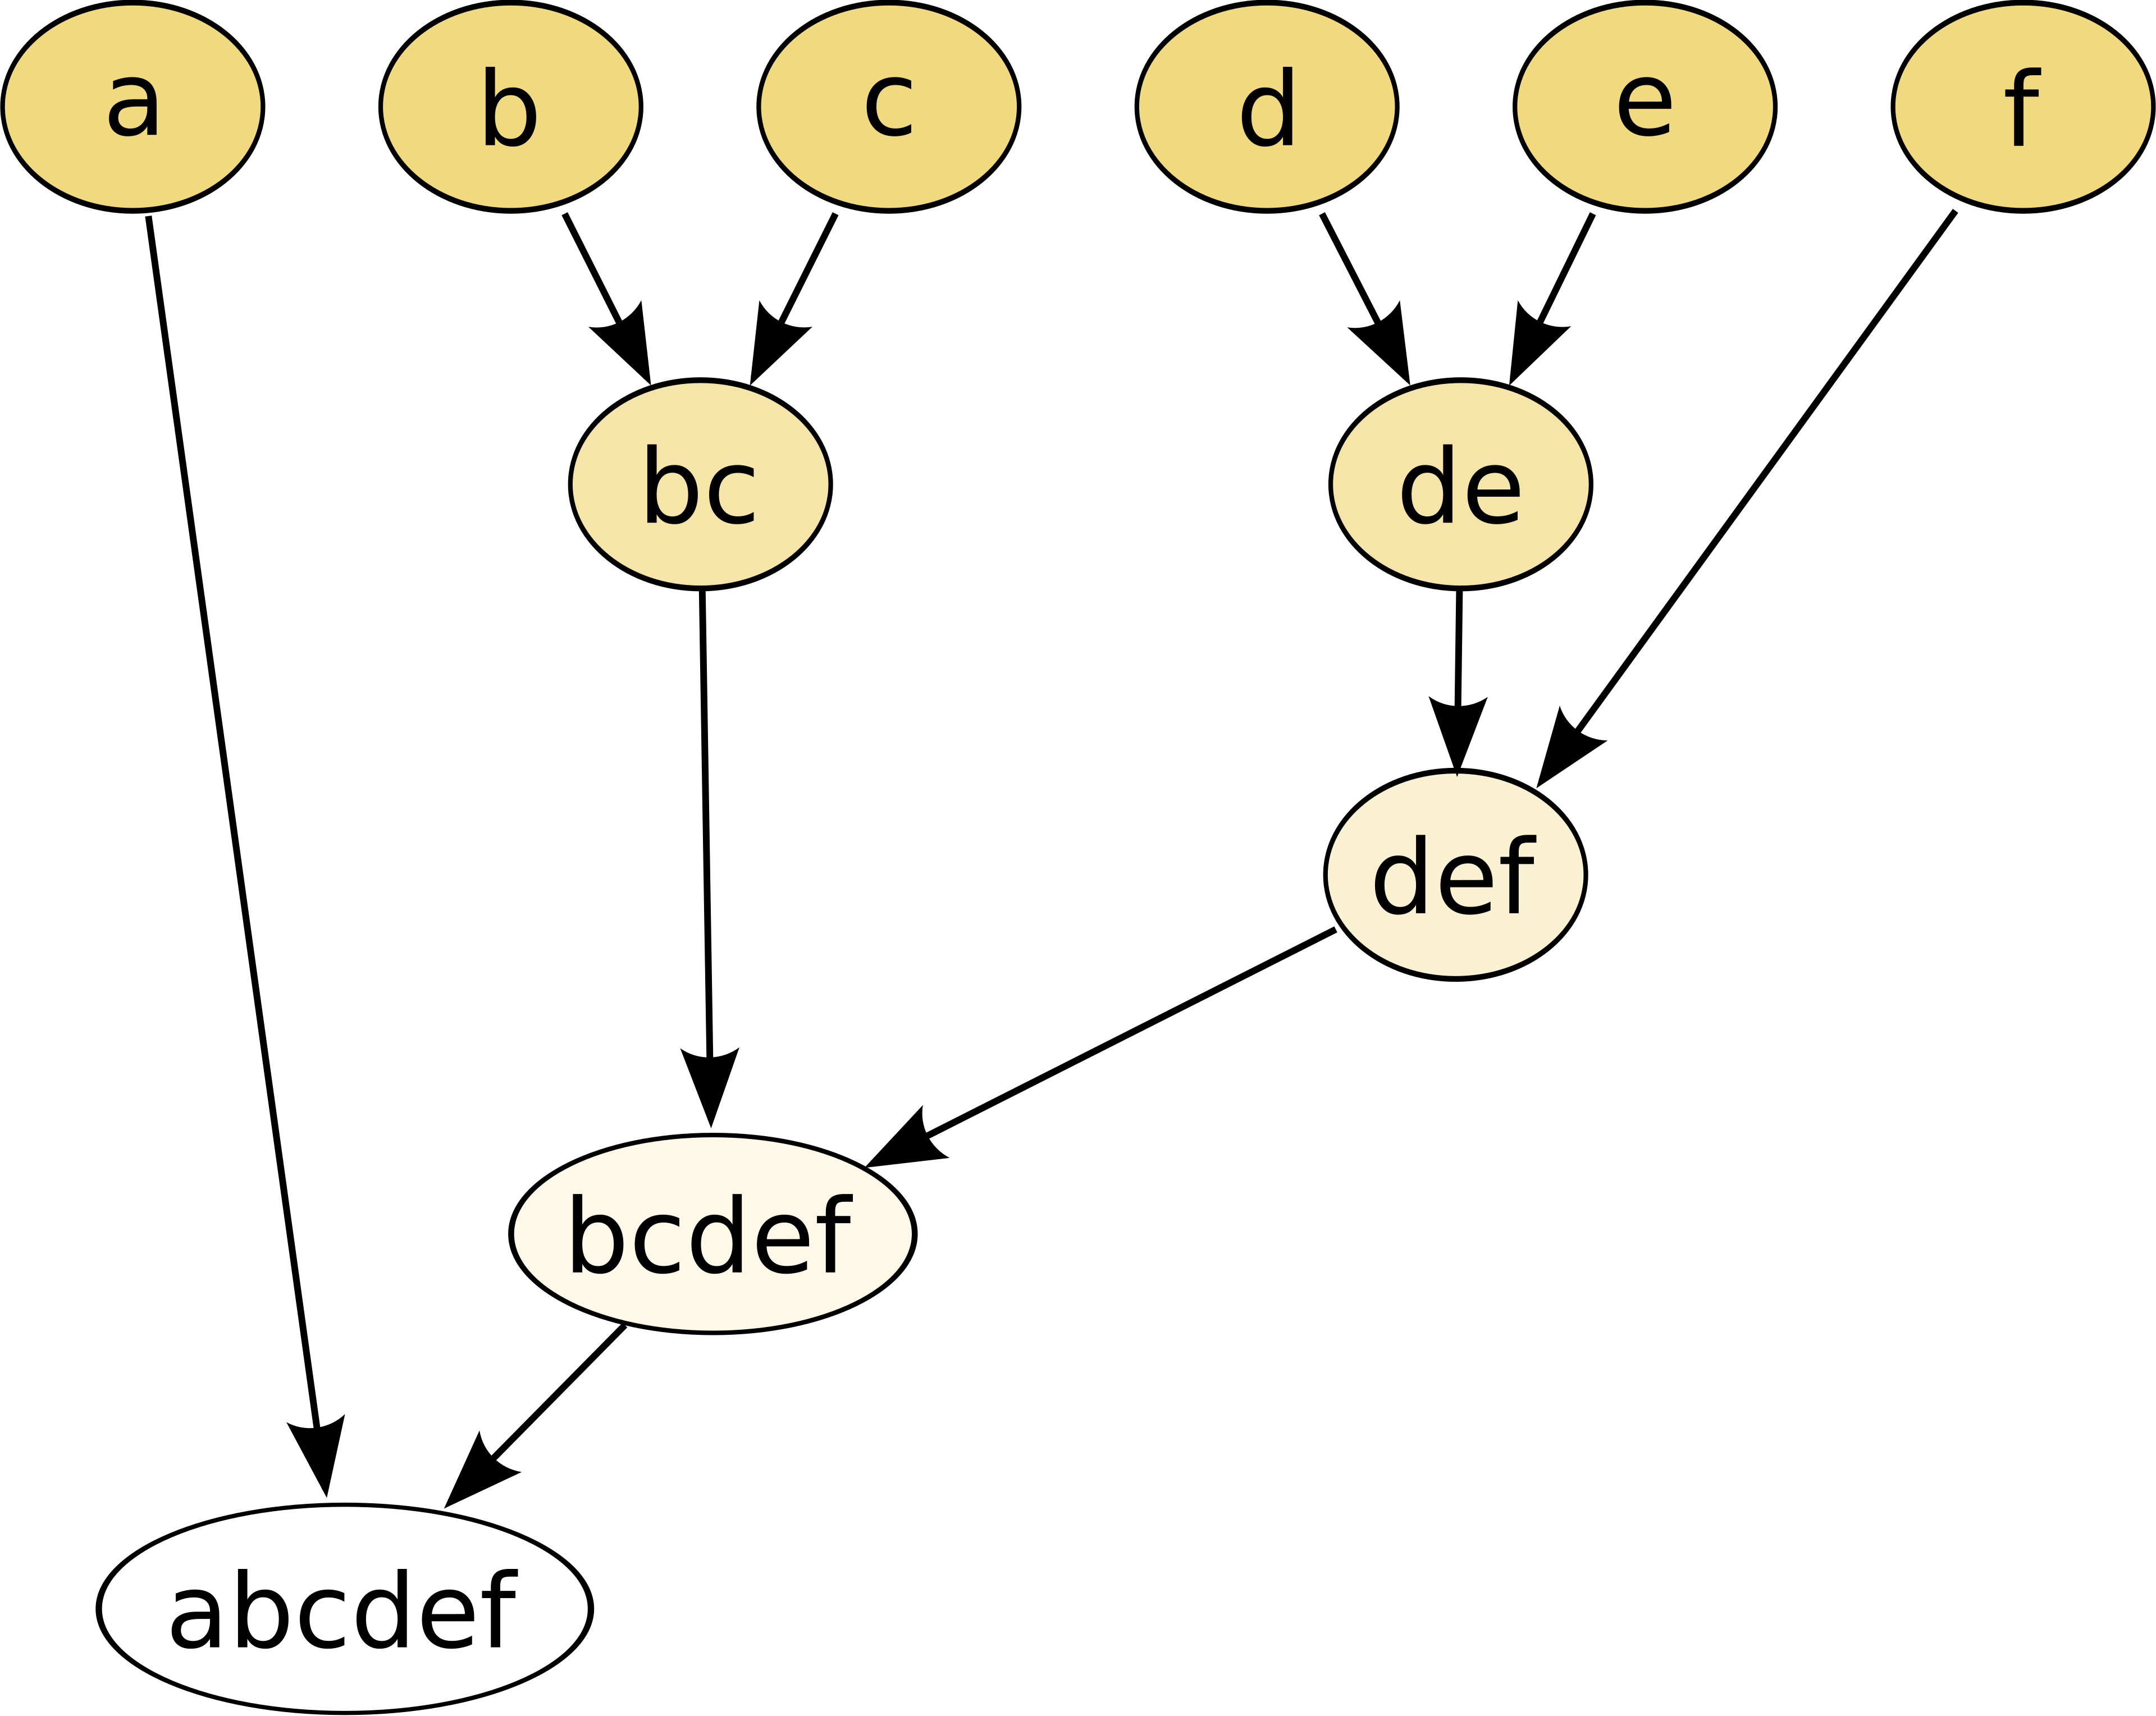
\includegraphics[width=0.5\linewidth]{figures_pedagogy/Hierarchical_clustering_simple_diagram.svg.png}
    \caption{An example dendrogram. Image credit: Mhbrugman (Wikipedia).}
    \label{fig:dendrogram}
\end{figure}

This type of clustering is very computationally expensive. You can expect it to take a long time to run on large datasets. But the method is very useful when you don't know how many clusters the data should have; making a dendrogram can help you visualize how many clusters there should be.


\clearpage
\section{Inferential Neural Networks}\label{sec:nn}
\subsection*{Learning Questions}
\begin{itemize}
    \item What is a perceptron?
    \item What is a multilayer perceptron?
    \item What is a ``feed-forward'' ``densely connected'' neural network?
    \item What is an RNN?
    \item What is LSTM?
    \item What is a CNN?
    \item What is regularization?
\end{itemize}

\subsection*{Introduction}
The neural network is an algorithm --- a collection of algorithms --- inspired by the human brain. A biological neuron receives signals through its dendrites, processes them in the cell body and sends the output through its axon. \textbf{Artificial neural networks} (ANNs) are simplified mathematical models of the biological process. They are a metaphor for the brain. The human (and not only human) brain has an uncanny ability to learn patterns and make connections between events. When ANNs were developing, the hope was that if we mimic \emph{the way} the brain learns with a computer, the computer can learn just as much, just as well, just as fast.

This lesson introduces \textit{inferential neural networks}, networks designed to make predictions from data. We will start with the simplest neural network, the perceptron, and then build up to modern architectures. We will cover densely connected neural networks for tabular data, recurrent neural networks (RNNs) for sequences, and convolutional neural networks (CNNs) for images. A discussion of generative neural networks (variational autoencoders, diffusion models, generative adversarial networks, transformers and large language models, all of which are now colloquially referred to as ``Artificial Intelligence'' (AI)) will come in the next lesson.

\subsection*{The Perceptron}
The \textbf{perceptron} is the simplest neural network. It was invented in 1957, though it was theorized a decade earlier. When the New York Times reported on it, they said that it would be able to read, write and even become conscious of its existence. It would take many decades for neural networks to learn to read and write, and their sentience is not even on the horizon.

Anyway. A perceptron is a binary classifier. It takes inputs, multiplies each input by a weight, sums the products, and then passes the result through a step function. If the output is above a threshold, the perceptron predicts one class; otherwise, it predicts the other.

Eventually, it was shown that such a simple algorithm could not only model linear functions. Everyone already knows how to model linear functions at this point, so the perceptron faded for a while. It was then discovered that multiple perceptrons \textit{would} be able to model nonlinearity. This is the multilayer perceptron, the foundation of modern deep learning.

\subsection*{The Neuron Equation}
A \textbf{neuron} is the fundamental unit of a neural network. Ultimately, a neuron is just a function. It has inputs and outputs. We can represent the inputs by a vector, $\mathbf{x}=[x_1,x_2,\ldots,x_n]$ and we can represent the output by a scalar, $y$. This function has parameters too, just like any other model we discussed. Normally, we referred to these parameters as $\boldsymbol{\beta}$, but in the context of ANNs, we will call them \textbf{weights,} which is also a vector, $\mathbf{w}=[w_1,w_2,\ldots,w_n]$. Do you recall how, in a linear model, there was always one more parameter than there were inputs? $p=n+1$. It's similar with the neuron: there is another parameter called the \textbf{bias} $b$. Thus we have $n$ inputs, $n$ weights, and $1$ bias. The last component of the neuron is its \textbf{activation function,} $f(z)$. The choice of activation function is a hyperparameter.

The neuron equation combines all of these elements into a simple equation:

\begin{align}
    y &= f \left( \mathbf{w} \cdot \mathbf{x} + b \right) \\
    y &= f \left( \sum_{i=1}^n w_i x_i + b \right)
\end{align}

\noindent The importance of this equation, not just for the field of machine learning and data science but for world history too, is nearly impossible to overstate.

\subsection*{Activation Functions}
The activation function is what gives ANNs their nonlinearity and thus their ability to learn complex relationships between inputs and outputs. The most widely used activation function is likely the \textbf{Rectified Linear Unit} (ReLU). It's defined simply as $f(z)= \max(0,z)$ where $z=\mathbf{w} \cdot \mathbf{x} + b$. If $z$, that combination of inputs, weights, and bias is less than zero, ReLU outputs a zero. If $z>0$, ReLU simply outputs $z$. This function is very computationally efficient and is generally the default, first choice activation function if you are unsure what to use.

The second most widely used activation function is likely the \textbf{sigmoid.} We've actually seen the sigmoid before --- it's the logistic function, $\sigma(z)=\frac{1}{1+e^{-z}}$. The input of the sigmoid can be any real number, but the output is always between zero and one.

\subsection*{The Multilayer Perceptron}
A single neuron is limited, but multiple neurons can learn anything. A \textbf{multilayer perceptron}  (MLP) consists of a group of neurons called the input layer, one or more groups of neurons called hidden layers, and one group of neurons called the output layer. In a \textbf{densely connected} (or fully connected) layer, every neuron in the layer receives input from every neuron in the previous layer. Each connection has it's own weight, and each neuron has its own bias.

\begin{figure}
    \centering
    
\includegraphics[width=0.5\linewidth]{Colored_neural_network.svg.png}
    \caption{ A simple Artificial Neural Network diagram of a densely connected network. Source: Wikipedia, Colin M.L. Burnett.}
    \label{fig:pedagogy_ann}
\end{figure}

Take a look at \autoref{fig:pedagogy_ann}, which shows an example of a densely connected neural network with one hidden layer. The input layer has three neurons, the hidden layer has four neurons, and the output layer has two neurons. How many parameters does this model have?

Let's construct a simple example. We have a dataset with three features and two targets.\footnote{We've only ever had datasets with one target feature before, but when you have more than one, it's called ``multi-label classification.''} Each of the three features is given as input to one of the three input neurons. These input neurons don't really do anything. They don't have any weights or biases, and no activation function is applied. They just serve as starting points for each of the features in our dataset. You'll always have as many input neurons as you have features.

Because the network is densely connected, each input neuron is passed to each hidden layer; each hidden layer has three inputs. This hidden layer consists of full neurons now, so we can begin counting the parameters. Each neuron in the hidden layer has one weight for each input ($3$), and there are four neurons in this layer, so there are $3\cdot4=12$ weights. There is also one bias per neuron, so that's another four parameters. We then repeat this with the output layer: each neuron in the output layer has four inputs, so there are $4\cdot2=8$ weights, and there are two neurons in the layer, so there are two biases.

In total, that's $26$ parameters: 20 weights and 6 biases. That's a lot more than the two parameters of the simple linear model! In general, the number of parameters in the $i$-th \textit{layer} of a densely connected neural network, $p_i$, is

\begin{equation}
    p_i=(n_{i-1} \cdot n_i) + n_i
\end{equation}

\noindent where the $n_i$ is the number of neurons in the $i$-th layer, and $n_{i-1}$ is the number of neurons in the previous layer.

When someone talks about a ``simple'' neural network, or a ``dense network,'' they're most likely referring to an MLP.

\subsection*{The Universal Approximation Theorem}
In 1989, it was proven that a neural network with a single hidden layer (with a finite number of neurons in that layer) can approximate \textit{any} continuous function. This is the \textbf{universal approximation theorem}.\footnote{We could be a bit more precise here. The theorem states that for any given function and any desired accuracy ($\epsilon > 0$), there exists a network with a sufficiently large, but finite, number of neurons in its hidden layer to achieve that accuracy on a compact (closed and bounded) subset of $\mathbb{R}^n$ (\eg{} [0,1]). Also, the activation function has some requirements, namely, it cannot be linear (recall that the perceptron could only learn linear functions, partially because it lacked a nonlinear activation function). Finally, it is an \emph{existence} theorem, not a learnability theorem: it proves that such a network exists, but it does not prove that the training will actually find the correct weights, nor does it guarantee the network will generalize well to unseen data.} Of course, there is no guarantee that you will be able to create that model; the theorem does not provide a way to calculate how many neurons you need. If you've ever heard that neural networks can learn ``anything,'' that is not hyperbole. However, I would advise you to consider what that person is trying to convince you of, because neural networks aren't magic. They rely on good data and on good architectural choices, like how many neurons, which activation functions, which loss function, etc., just like any other model.

\subsection*{Training Neural Networks}
The goal of training a neural network is to adjust the weights and biases so that the output of the network matches the target output. Does this sound familiar? This is exactly like every other supervised machine learning model we've discussed. And just like those other models, the neural network needs an objective function. In the context of ANNs, you'll mostly hear them called ``loss functions.''

For regression tasks, you may use any of the objective functions we've discussed before. Mean Squared Error (MSE) is still the most common. For binary classification tasks, you'll want to use a version of the log loss utilized in logistic regression. This time it's called \textbf{binary cross-entropy}, but really it's the same thing. For multi-class classification\footnote{Multi-class classification is where you are predicting one target with multiple classes, \eg{} predicting whether an image is of an apple, banana, or peach. Binary classification is when you are predicting one target with only two classes. Multi-label classification is when you are predicting multiple \textit{targets}, \eg{} predicting whether an image contains fruit \textit{and} whether the image contains an animal.} the loss function is similar, but it's called \textbf{categorical cross-entropy}.\footnote{As it turns out, one can express a lot of creativity in the formulation of the loss function, and a lot of what makes a model successful is a good, perhaps custom-designed loss function. The ones listed above are the canonical choices which are all you will need to work with in this class, and perhaps in your whole data science career.}

\subsubsection*{Backpropagation}
It was a challenge figuring out the OLS method for finding the best parameters for the linear model, and the tiny network shown in \autoref{fig:pedagogy_ann} had 26 parameters! How do we find the best values for all those weights and biases? The algorithm is called \textbf{backpropagation}. First, the network passes the data through the network, calculating the neuron equation for every neuron in sequence. The model produces an output, and the objective function is used to calculate the loss on that output compared to the desired output. Then, the errors are propagated \textit{backwards} through the network. The details of backpropagation lie in complex calculus; essentially, the algorithm determines which parameter is responsible for increasing the loss on each output, and by how much (leveraging differentiation and the chain rule). The parameter is then updated to lower the loss, and all of that represents one \textbf{batch} of learning.

A batch can include one observation passing through the network; it can include the entire training set passing through the network, or it can (and in most cases does) include some amount in between. The \texttt{batch\_size} hyperparameter governs this for most implementations of ANNs.

\subsection*{Recurrent Neural Networks}
Feed-forward neural networks treat each input independently. The neuron doesn't store any information about what it has done in the past. This works great for tabular data, but many tasks involve sequential data: time series, text, audio and video. A \textbf{recurrent neural network} (RNN) processes each element of the sequence in order, rather than all at once. The RNN introduces the concept of a hidden state. At each element, the RNN saves some information in that hidden state variable. At the next element, the hidden state information from the previous element is provided. The model produces an output and a new hidden state, and the cycle repeats. This hidden state is like the memory of the network.

Consider a time series of daily temperatures. You want to predict tomorrow's temperature based on the past week. An RNN processes the sequence day by day. At each step, it updates its hidden state based on the temperature of that day and the previous hidden state. At the final step, the hidden state contains information about the entire sequence, and the network produces a prediction for tomorrow.

The RNN as described suffers from an issue called the \textbf{vanishing gradient problem.} When the sequence is long, the gradients (the part of the backpropagation algorithm that propagates errors through the model) can become so small that they ``vanish.'' This means that RNNs struggle with long sequences.

The solution is the \textbf{long short-term memory} (LSTM) network. The LSTM introduces a \textbf{cell state} that runs through the entire sequence, \textbf{gates} that control the flow of information. The details are interesting but beyond the scope of this lesson. Suffice it to say that LSTMs are the de facto standard ANN for sequential data, though this has changed since 2017 with the advent of the Transformer, which we will discuss in the next lesson.

\subsection*{Convolutional Neural Networks}
None of the networks discussed so far were designed with images in mind. Images are tricky. They are at least 2D (height, width), but they can be three or four dimensional (height, width, color, transparency/depth). On top of that, images have spatial structure; neighboring pixels are related. The MLP would ignore this structure, treating each pixel as an independent feature. A \textbf{convolutional neural network} (CNN) is designed for 2D data and includes the spatial structure in its calculations.

The CNN uses the convolution operation to extract features from images. The convolution starts with a filter (also called a kernel) that slides over the image. For example, consider an image that is five pixels by five pixels and a kernel that is three pixels by three pixels. We can represent them with matrices.

\begin{align}
    \text{Image}=
    \begin{bmatrix}
        a_{11} & a_{12} & a_{13} & a_{14} & a_{15} \\
        a_{21} & a_{22} & a_{23} & a_{24} & a_{25} \\
        a_{31} & a_{32} & a_{33} & a_{34} & a_{35} \\
        a_{41} & a_{42} & a_{43} & a_{44} & a_{45} \\
        a_{51} & a_{52} & a_{53} & a_{54} & a_{55}
    \end{bmatrix}
    \quad
    \text{Kernel}=
    \begin{bmatrix}
        k_{11} & k_{12} & k_{13} \\
        k_{21} & k_{22} & k_{23} \\
        k_{31} & k_{32} & k_{33}
    \end{bmatrix}
\end{align}

\noindent where $a_{ij}$ is the image pixel value at row $i$ and column $j$, and $k_{ij}$ are the kernel pixel values.

When we say that the kernel ``slides'' over the image, imagine that the kernel is overlaying on top of the image. The kernel starts in the top left of the image, represented here by the $3 \times 3$ sub-matrix.

\begin{equation*}
    \begin{bmatrix}
        a_{11} & a_{12} & a_{13}\\
        a_{21} & a_{22} & a_{23}\\
        a_{31} & a_{32} & a_{33}
    \end{bmatrix}
\end{equation*}

\noindent Then the sub-matrix and the kernel are multiplied together, element-wise, and all of the elements are added together. This results in one element, $c_{11}$, of the result of the convolution. The kernel slides over the image, combining with the sub-matrices to fill out the resulting convolution.

\begin{align}
    \text{Convolution}=
    \begin{bmatrix}
        c_{11} & c_{12} & c_{13}\\
        c_{21} & c_{22} & c_{23}\\
        c_{31} & c_{32} & c_{33}
    \end{bmatrix}
\end{align}

That was pretty abstract, so let's try that again with actual numbers. Given the following image and kernel, what is the resulting convolution?

\begin{align}
    \text{Image}=
    \begin{bmatrix}
        1 & 0 & 0 & 0 & 1 \\
        0 & 1 & 0 & 1 & 0 \\
        0 & 0 & 1 & 0 & 0 \\
        0 & 1 & 0 & 1 & 0 \\
        1 & 0 & 0 & 0 & 1
    \end{bmatrix}
    \quad
    \text{Kernel}=
    \begin{bmatrix}
        1 & 0 & 0 \\
        0 & 1 & 0 \\
        0 & 0 & 1
    \end{bmatrix}
\end{align}

\noindent The first three sub-matrices that the kernel would combine with are:

\begin{align}
    \begin{bmatrix}
        1 & 0 & 0 \\
        0 & 1 & 0 \\
        0 & 0 & 1 
    \end{bmatrix}\quad
    \begin{bmatrix}
        0 & 0 & 0\\
        1 & 0 & 1\\
        0 & 1 & 0
    \end{bmatrix}\quad
    \begin{bmatrix}
        0 & 0 & 1 \\
        0 & 1 & 0 \\
        1 & 0 & 0
    \end{bmatrix}.
\end{align}

\noindent When we perform the element-wise multiplication with the kernel and then sum all the elements, we get:

\begin{align}
    \begin{bmatrix}
        1 & 0 & 0 \\
        0 & 1 & 0 \\
        0 & 0 & 1 
    \end{bmatrix}\rightarrow3 \quad
    \begin{bmatrix}
        0 & 0 & 0\\
        0 & 0 & 0\\
        0 & 0 & 0
    \end{bmatrix}\rightarrow0 \quad
    \begin{bmatrix}
        0 & 0 & 0 \\
        0 & 1 & 0 \\
        0 & 0 & 0
    \end{bmatrix}\rightarrow1.
\end{align}

\noindent Repeating this for all nine sub-matrices, the result of the convolution is

\begin{align}
    \text{Convolution}=
    \begin{bmatrix}
        3 & 0 & 1 \\
        0 & 3 & 0 \\
        1 & 0 & 3 
    \end{bmatrix}.
\end{align}

The original image was an x-shape, the kernel was a diagonal line going down to the right, and the final convolution was another x-shape with a diagonal line emphasized. This example demonstrates what convolutions do. \textbf{The convolution finds shapes in the image that are similar to the shape in the kernel}.

The CNN incorporates several convolutional layers, each with several different kernels working in parallel, to extract parts of the input that look like the kernel. We call the result of these convolutions ``feature maps.'' The trick with the CNN is that the parameters in a convolutional layer are the pixels of the kernel. As the CNN learns, the shape of the kernels changes, and the features extracted from the inputs are adjusted based on what would produce the best output for the model.

\subsection*{Regularization}
Because neural networks are so flexible, they're prone to overfitting. The universal approximation theorem already tells us that a network with only one dense layer can learn any function. If you have a network with many dense layers, with many neurons each, its very easy for a network to learn the training data so well that it fails to generalize to anything else. \textbf{Regularization} is the term for the set of techniques that aim to improve generalizability in machine learning models. For ANNs, regularization is often necessary.

\textbf{Dropout} is a regularization technique that forces a fraction of the neurons in a network to set their output to zero. This forces the network to learn multiple representations of the data, which helps the model generalize. The dropout rate is a hyperparameter. Another form of regularization is \textbf{early stopping.} During training, we are always monitoring how the loss function performs on the validation set. If the loss on the validation set stops improving or starts worsening, early stopping will halt training. When the validation set performance stops improving, that's a good indicator that the model's generalizability isn't improving either.

\subsection*{The Black Box}
Neural networks are referred to as ``black boxes.'' They often have so many parameters that it's impossible to interpret why a particular prediction was made. Contrast this with a decision tree classifier, and it's immediately obvious what decisions were made that led to a prediction. This critique is valid, but it's not always a problem. Neural networks achieve state-of-the-art performance on many tasks --- that's why they're so popular; they're demonstrably powerful. But if interpretability is important, which it is in some domains like medicine or criminal justice, then ANNs may not be appropriate.


\clearpage
\section{Generative Neural Networks}
\subsection*{Learning Questions}
\begin{itemize}
    \item What is the difference between an inferential and generative neural network?
    \item What is an autoencoder?
    \item What is a variational autoencoder?
    \item What is the latent space?
    \item What is a generative adversarial network?
    \item What is a diffusion model?
    \item What is the Transformer?
    \item What is the attention mechanism?
    \item What is a large language model?
\end{itemize}

\subsection*{Introduction}
In the last lesson, we explored inferential neural networks, models that make predictions from data. For example, a neural network can be trained on a dataset of handwritten digits so that it can classify what digit an image contains. The model's input is an image, and its output is a label. But what if we want to create new data instead of classifying (or regressing) it? What if we want to generate a new image of a handwritten digit that doesn't exist in the training set? This is the domain of \textbf{generative neural networks.}

Generative models learn the underlying distribution of the training data. Once trained, they can sample from this distribution to create new data that ``resembles'' (or is consistent with) the training set. Generative models can produce images, text, music and video that appear human-made. This is its greatest strength, but it also presents the greatest dilemma, which we will discuss at the end of the lesson.

\subsection*{Autoencoders}
An \textbf{autoencoder} is a neural network that learns to reconstruct its input. It consists of two components: an encoder and a decoder, which can almost be considered two separate models. The encoder takes the input data and compresses it into a lower-dimensional representation called the \textbf{latent space.} The decoder takes this compressed representation and reconstructs the original input. Just like any model, this one needs a loss: the network is trained to minimize the difference between the input and the reconstruction --- the reconstruction loss.

Consider a dataset of handwritten digits. One such popular dataset exists called the \texttt{MNIST} dataset. Each image in the dataset is $28 \times 28\text{ pixels}$. An autoencoder for \texttt{MNIST} might have an encoder that compresses the image represented by $28\times28=784\text{ numbers}$ into just $16$ numbers. These $16$ numbers constitute the latent space. The decoder then takes those $16$ numbers and reconstructs a $28 \times 28\text{ pixel}$. The network learns to preserve the most important features of the digits, \eg{} its shape, the width of each line, the orientation, etc. \autoref{fig:vae} shows an example architecture diagram of an autoencoder.

\begin{figure}
    \centering
    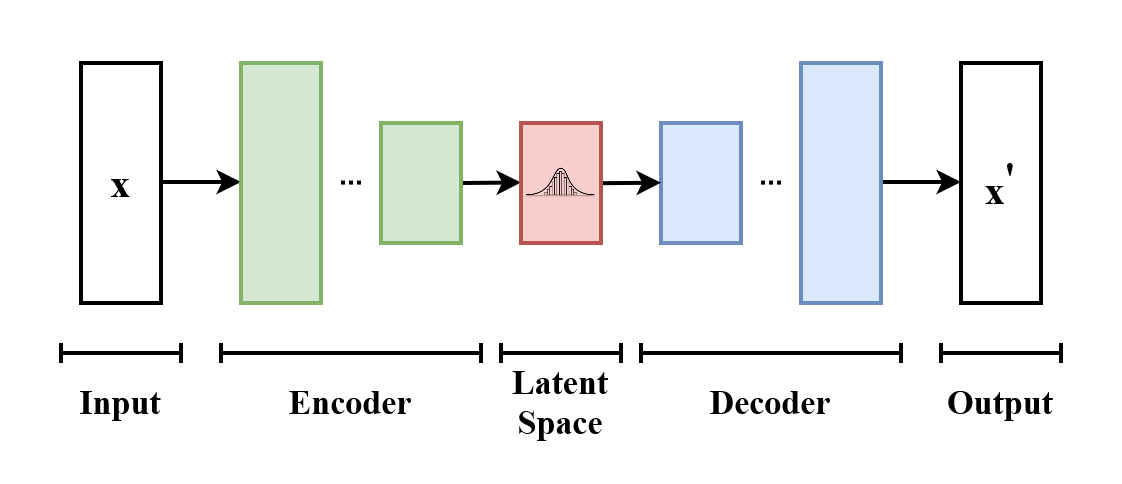
\includegraphics[width=1\linewidth]{figures_pedagogy/VAE_Basic.png}
    \caption{An example (variational) autoencoder architecture. Image credit: EugenioTL (Wikipedia)}
    \label{fig:vae}
\end{figure}

We talked before about how convolutional neural networks (CNNs) are particularly well-suited to dealing with image data. Thus, you may imagine that an autoencoder could make use of convolutions too. The convolution can certainly be used to create this latent space. However, what operation do we use to increase the dimensions of the data from the latent space? This is done using the transpose of the convolution operation. Transposed convolution (sometimes called ``deconvolution''\footnote{The term ``deconvolution'' does not actually refer to a transposed convolution, though the two terms are often used interchangeably. Avoid using ``deconvolution.''}) increases the size of the image, rather than decreases it as the convolution operation does. Transposed convolution learns the best way to increase the resolution from the data.

The autoencoder can be extended to perform more advanced tasks. For example, we can mask parts of the input --- either random pixels or entire regions are hidden from the model during training --- and train the network to reconstruct the full image from the partial input. This forces the network to learn a richer representation of the data. Or we can train it to improve the resolution or quality of an image (Instagram and TikTok filters that do this could very well be based on this technology).

\subsection*{Variational Autoencoders}
A standard autoencoder learns a deterministic mapping from input to latent space. Given an input, the encoder always produces the same latent representation. This works for reconstruction, but it makes generation difficult. If we observe the distribution of values that the latent space takes for each digit, then we can sample from those distributions, feed them into the decoder, and then produce an entirely new image of a digit. But if we do this, we may end up choosing latent space parameters that do not correspond to any real data.

The \textbf{variational autoencoder} (VAE) solves this problem by learning a probability distribution over the latent space. Instead of outputting a single point, the encoder outputs a mean and a variance for each latent dimension. The decoder then samples from this distribution to generate new data.

The VAE has a special loss function with two components. The reconstruction loss term measures how well the decoder reconstructs the input, but the \textbf{KL divergence} term measures how close the learned latent distribution is to a standard normal distribution. The Kullback–Leibler (KL) divergence is a measure of how one probability distribution differs from another. This term penalizes the model during training if the latent space is not smooth and continuous. This allows us to then sample from the latent space and generate new data that looks plausible. If a VAE were trained on the \texttt{MNIST} dataset, we could sample the latent space at different points to generate images of digits drawn with different styles.

\subsection*{Generative Adversarial Networks}
A \textbf{generative adversarial network} (GAN) takes a different approach to generation. Instead of learning a latent space, a GAN uses two networks that compete against each other. The \textbf{generator} creates fake data from random noise. The \textbf{discriminator} tries to distinguish real data from fake data. The two networks are trained together in an adversarial game. The generator creates images with the express purpose of trying to fool the discriminator. Over time, the generator becomes better at creating realistic data as the discriminator becomes better at detecting fakes.

For \texttt{MNIST}, the generator takes a random noise vector as input and outputs a $28 \times 28$ image of a digit. The discriminator receives both real \texttt{MNIST} images and generated images, and tries to classify them as real or fake. As training progresses, the generator learns to produce images that look like real digits.

GANs can produce high-quality, realistic images, but the training can be unstable. The generator may suffer from \textit{mode collapse,} where it produces only a few types of outputs.

\subsection*{Diffusion models}
\textbf{Diffusion models} work by gradually adding noise to data and then learning to reverse the process. In the \textbf{forward process,} noise is added to an image step-by-step. After enough steps, the image becomes only random noise. In the \textbf{reverse process,} the model learns to remove the noise step by step, recovering the original image. Once trained, a diffusion model can generate new images by starting with pure random noise and iteratively applying the learned denoising process. After enough steps, the noise becomes a coherent image.

Diffusion models produce high-quality, diverse outputs and are more stable to train than GANs. However, they are also slow to generate images because they require many iterative steps.

\begin{figure}
    \centering
    
\includegraphics[width=0.5\linewidth]{figures/evaluateGAI.png}
    \caption{The strengths and weaknesses of each of the three main generative AI frameworks: Variational Autoencoders and Normalizing Flows, Generative Adversarial Networks, and Diffusion Models. From \url{https://www.nvidia.com/en-us/glossary/generative-ai/}.}
    \label{fig:genai}
\end{figure}

\subsection*{VAE, GAN or Diffusion?}
The previous sections contained guidance on the pros and cons of three generative AI approaches commonly used for image generation. \autoref{fig:genai} conveys these pros and cons graphically to help you choose what to use based on your requirements on accuracy, diversity of generated data, and computational constraints.

\subsection*{Transformers}
Generative models are not limited to images. How can models be trained to generate realistic sentences? Language is sequential and structured; the meaning of a word depends on the words around it. As we discussed earlier in this chapter, recurrent neural networks (RNNs) can work with sequential data, but they struggle to deal with long-range dependencies (\ie{} the effect of words that are separated from each other by many words) without long short-term memory (LSTM). The \textbf{Transformer} architecture solved this problem in another way.

The key innovation of the Transformer is the \textbf{attention mechanism.} Attention allows a model to focus on the relevant parts of the input. For text, attention lets each word ``look at'' all other words in the sequence. This captures relationships between distant words. For example, in the sentence ``The cat that chased the mouse was hungry,'' attention helps the model connect ``was'' with ``cat'' even though many words separate them.

The original Transformer has an encoder-decoder structure. The encoder processes the input sequence, and the decoder generates the output sequence. Some models only use the decoder. These decoder-only models (like GPT) are designed for autoregressive generation. They process the input sentence and generate the output one word at a time.\footnote{These models don't process words but ``tokens,'' mathematical representations of words or word fragments.} The model predicts the next word in the sequence based on all previous words.

Consider the sentence: ``The quick brown fox jumps over the lazy.'' One such language model could learn to predict the next word, ``dog,'' based on the text of the sentence and the context it learned throughout training. Indeed, such a model could continue predicting words forever.

\subsection*{Foundation Models and Pretraining}
A \textbf{foundation model} is a large neural network\footnote{``Large'' meaning many parameters.} trained on a massive dataset on a reconstruction task (\eg{} regenerating the data, like we have seen in the autoencoder case or reconstructing missing pixels in images). This way, these models learn general patterns and relationships among the data, and then the models are adapted to many different tasks.

\textbf{Pretraining} is the process of training a model on a large, general dataset before fine-tuning it for a specific task. For example, a language model can be trained on billions of words from the internet, and after this pretraining, it can be \textbf{fine-tuned} on a smaller dataset for a specific task. For example, you can pretrain on a British English corpus and fine-tune on an American English corpus. Or you can pretrain on a large corpus of artwork and fine-tune on Andy Warhol alone to generate art in his style (we will address ethical implications in a moment).

\textbf{Large language models} (LLMs) are foundation models for text. They can generate human-like text, answer questions and even write code. They are the result of scaling up the Transformer architecture to enormous sizes. GPT, Claude, Grok, Gemini and DeepSeek are all examples of LLMs.

\subsection*{Ethics of Generation}
Generative models raise significant ethical concerns. They learn from human data --- our text, our images, etc. --- which contains human biases. These biases can be amplified by the model, leading to harmful outputs when generative models are applied to tasks like hiring, law enforcement, healthcare and translation. Gender and racial biases are some of the most visible biases in these models, where they will make obviously harmful assumptions about people based on their race and gender. These stereotypes exist in the modern world, and these training sets are so large that it's impossible to completely de-bias them.

Generative models are often misused to lie and mislead. They can create a convincing fake news post, advertisement or video so quickly and easily. The existence of these models threatens public trust in the world around them.

Most generative models are trained on data scraped from the internet without permission (from the website or from the authors). This includes copyrighted works, personal data, and art. It's now possible for an artist's entire portfolio to be uploaded to the dataset of a generative image model, and then ask the model to produce a new image in that artist's style. The data \textit{is} the model. If the data is stolen, then any output of the model represents theft.

